%
% Niniejszy plik stanowi przykład formatowania pracy magisterskiej na
% Wydziale MIM UW.  Szkielet użytych poleceń można wykorzystywać do
% woli, np. formatujac wlasna prace.
%
% Zawartosc merytoryczna stanowi oryginalnosiagniecie
% naukowosciowe Marcina Wolinskiego.  Wszelkie prawa zastrzeżone.
%
% Copyright (c) 2001 by Marcin Woliński <M.Wolinski@gust.org.pl>
% Poprawki spowodowane zmianami przepisów - Marcin Szczuka, 1.10.2004
% Poprawki spowodowane zmianami przepisow i ujednolicenie 
% - Seweryn Karłowicz, 05.05.2006
% Dodanie wielu autorów i tłumaczenia na angielski - Kuba Pochrybniak, 29.11.2016

% dodaj opcję [licencjacka] dla pracy licencjackiej
% dodaj opcję [en] dla wersji angielskiej (mogą być obie: [licencjacka,en])
\documentclass[licencjacka]{pracamgr}


% Dane magistranta:
\autor{Urszula Papiernik}{448554}


% Dane magistrantów:
%\autor{Urszula Papiernik}{448554}

\title{Wymiar Pokryciowy: charakteryzacja za pomocą $\varepsilon$-przekształceń}


\tytulang{ Covering Dimension: characterization via $\varepsilon$-mappings }

%kierunek: 
% - matematyka
% - Mathematics
\kierunek{matematyka}

% informatyka - nie okreslamy zakresu (opcja zakomentowana)
% matematyka - zakres moze pozostac nieokreslony,
% a jesli ma byc okreslony dla pracy mgr,
% to przyjmuje jedna z wartosci:
% {metod matematycznych w finansach}
% {metod matematycznych w ubezpieczeniach}
% {matematyki stosowanej}
% {nauczania matematyki}
% Dla pracy licencjackiej mamy natomiast
% mozliwosc wpisania takiej wartosci zakresu:
% {Jednoczesnych Studiow Ekonomiczno--Matematycznych}

% \zakres{Tu wpisac, jesli trzeba, jedna z opcji podanych wyzej}

% Praca wykonana pod kierunkiem:
% (podać tytuł/stopień imię i nazwisko opiekuna
% Instytut
% ew. Wydział ew. Uczelnia (jeżeli nie MIM UW))
\opiekun{dr. Andrzeja Nagórko
  }

% miesiąc i~rok:
\date{Maj 2026}

%Podać dziedzinę wg klasyfikacji Socrates-Erasmus:
\dziedzina{ 
%11.0 Matematyka, Informatyka:\\ 
11.1 Matematyka\\ 
%11.3 Informatyka\\ 
}

%Klasyfikacja tematyczna wedlug AMS (matematyka) lub ACM (informatyka)
\klasyfikacja{
  54 General Topology\\
  54F45 Dimension theory in general topology
  % D. Software\\
  % D.127. Blabalgorithms\\
  % D.127.6. Numerical blabalysis
  }

% Słowa kluczowe:
\keywords{
  wymiar pokryciowy, wielościany, $\epsilon$-przekształcenia, 
% blabaliza różnicowa, fetory $\sigma$-$\rho$, fooizm,
  % blarbarucja, blaba, fetoryka, baleronik
  }

% Tu jest dobre miejsce na Twoje własne makra i~środowiska:
\usepackage{amssymb}
\usepackage{amsmath}
\usepackage{amsthm}
\usepackage{graphicx}
\usepackage{float}
\usepackage{svg}
\usepackage{tikz}
\usepackage{tikz-3dplot}

\usepackage[
    backend=biber,
    style=numeric,
    sorting=none
]{biblatex}
\addbibresource{bibliografia.bib}
\usepackage[hidelinks]{hyperref}

\DeclareMathOperator{\ord}{ord}
\DeclareMathOperator{\St}{St}
\DeclareMathOperator{\ind}{ind}
\DeclareMathOperator{\Ind}{Ind}
\DeclareMathOperator{\Fr}{Fr}


\newtheorem{defi}{Definicja}[chapter]
\newtheorem{twie}[defi]{Twierdzenie}
\newtheorem{wnio}[defi]{Wniosek}
\theoremstyle{definition}
\newtheorem{przy}[defi]{Przykład}

% koniec definicji

\begin{document}

\maketitle

%tu idzie streszczenie na strone poczatkowa
\begin{abstract}
  W pracy omawiane jest pojęcie wymiaru pokryciowego zdefiniowanego przy pomocy krotności pokryć przestrzeni. Celem pracy jest charakteryzacja przestrzeni o wymiarze pokryciowym co najwyżej $n$, poprzez utorzsamianie ich za pomocą $\varepsilon$-przekształceń z co najwyżej $n$ wymiarowymi wielościanami, zdefiniowanymi przez $l$-wymiarowe sympleksy. W pracy omawiane jest również pojęcie nerwu pokrycia oraz funkcji $\kappa$-kuratowskiego.
\end{abstract}

\tableofcontents
%\listoffigures
%\listoftables

\chapter*{Wprowadzenie}
Teoria wymiaru jest jedną z dziedzin topologii, formalizujca tak zwane pojęcie „wymiaru“ przestrzeni topologicznej. Polega na przypisaniu każdej przestrzeni pewnej liczby, która zgodnie z naszą intuicją mówi, jak „duża“ jest dana przestrzeń. Najczęściej omawiane są mały wymiar indukcyjny, wymiar pokryciowy oraz duży wymiar indukcyjny.

Jednymi z najważniejszych osiągnięć teori wymiaru, jest pokazanie równości $\dim I^n=n$ \cite{bro1913} czego istotnym rezultatem jest pokazanie zależności $n\neq m \Longrightarrow \mathbb{R}^n\not \cong \mathbb{R}^m $, czyli że przestrzenie euklidesowe różnych wymiarów nie są homeomorficzne. W teorii wymiaru najczęściej rozważa się trzy funkcje: wymiar pokryciowy $\dim$, mały wymiar indukcyjny $\ind$ oraz duży wymiar indukcyjny $\Ind$. Dla przestrzeni metrycznych ośrodkowych zachodzi $ \dim X = \ind X = \Ind X.$ W ogólności równość ta nie jest spełniona.
Do ważnych osiągnięć należą też twierdzenia:
$\dim (X \cup Y) \le \dim X + \dim Y + 1$, czyli że suma dwóch przestrzeni zwiększa wymiar o co najwyżej jeden oraz $\dim (X \times Y) \le \dim X + \dim Y$, czyli wymiar iloczynu kartezjańskiego
nie przekracza sumy wymiarów.

Tematem tej pracy jest wymiar pokryciowy, który został poraz pierwszy wprowadzony przez Henri Lebesque'a \cite{lebesque1921}, a zformalizowany przez Eduarda Čecha \cite{cech1993}. 

W pierwszym rozdziale wprowadzimy definicję wymiaru pokryciowego, twierdzenie pozwalające nam zoptymalizować poszukiwanie go oraz wspomnimy o małym i dużym wymiarze powierzchniowym. W drugim rozdziale zdefiniujemy sympleksy oraz wielościany. Trzeci rozdział poświęcony będzie nerwom pokrycia, a w rodziale czwartym udowodnimy cel pracy, czyli twierdzenie o charakteryzacji przestrzeni topologicznych za pomocą $\varepsilon$-przekształceń. Głównym źródłem był podrzęcznik napisany przez Ryszarda Engelkinga \cite{engelking1995}.
\addcontentsline{toc}{chapter}{Wprowadzenie}

\chapter{Wymiar pokryciowy}
W całej pracy jako przestrzeń rozumiemy przestrzeń metryczną i ośrodkową. 
\section{Podstawowe definicje}
Zanim przejdziemy do pokazania definicji wymiaru pokryciowego, zacznijmy od przypomnienia i wprowadzenia kilku definicji pomocniczych.

\begin{defi}
    Jeżeli przestrzeń $X$ spełnia:
    dla każdej pary zbiorów domkniętych $A, B \subset X$ spełniających $A\cap B=\emptyset$, istnieją takie otwarte zbiory $U, V\subset X$, że $A\subset U$, $B\subset V$, $U\cap V=\emptyset$, to powiemy że $X$ jest przestrzenią \emph{normalną}.
\end{defi}
Podana własność często jest również nazywana własnością \emph{T4}. Dla przypomnienia, własnością \emph{T2}, czyli przestrzeń Hausdorffa, nazywamy możliwość oddzielenia dwóch punktów przez otoczenia otwarte, a własnością \emph{T3}, czyli przestrzeń regularną, możliwość oddzielenia punktów od zbiorów domkniętych przez otoczenia otwarte. 
\begin{defi}
    Powiemy, że przestrzeń jest \emph{zwarta}, jeżeli z każdego otwartego pokrycia możemy wybrać podpokrycie skończone.
\end{defi}

\begin{defi}
    Pokrycie $\mathcal{B}$ jest \emph{wpisaniem} pokrycia $\mathcal{A}$ tej samej przestrzeni $X$, jeżeli dla każdego $B\in \mathcal{B}$ istnieje $A\in \mathcal{A}$, takie że $B\subset A$.
    \begin{figure}[H]
        \centering
        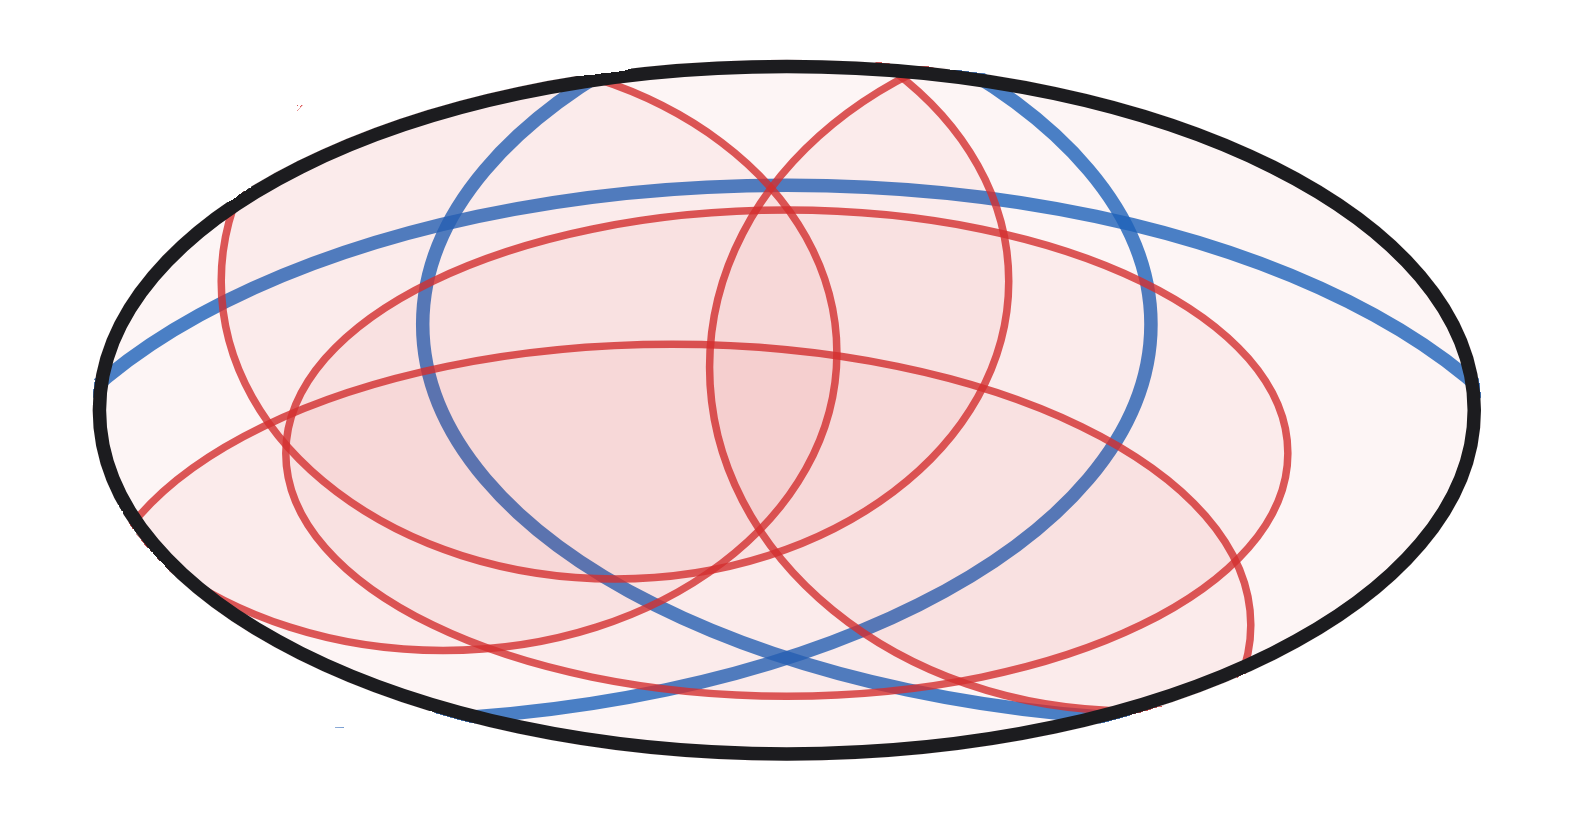
\includegraphics[width=0.5\textwidth]{pictures/wpisanie_przy.png}
        \caption{wpisanie}
        \label{fig:wpis}
    \end{figure}
\end{defi}
\begin{defi}
    \emph{Zwężeniem} pokrycia $\{A_s\}_{s\in S}$ przestrzeni $X$ nazwiemy pokrycie $\{B_s\}_{s\in S}$ przestrzeni $X$ spełniające $\forall_{s\in S} B_s \subset A_s$.
    \begin{figure}[H]
        \centering
        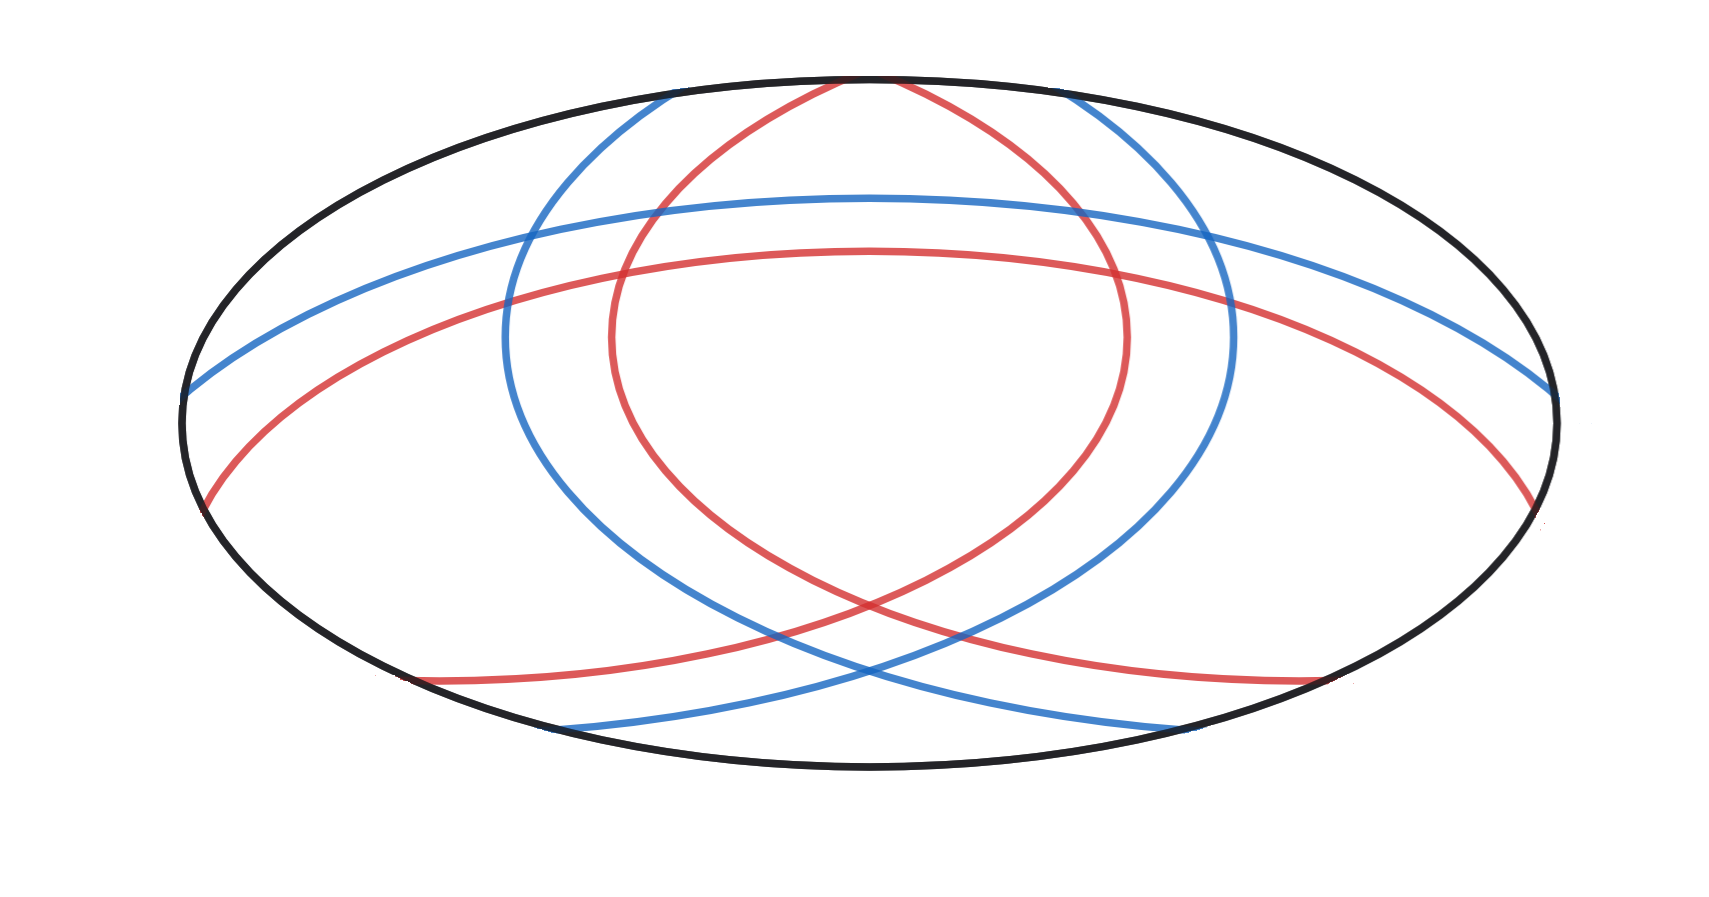
\includegraphics[width=0.5\textwidth]{pictures/zwerzenie_przy.png}
        \caption{zwężenie}
        \label{fig:zwerz}
    \end{figure}
\end{defi}
Zauważmy, że oczywiście każde zwężenie jest również wpisaniem.

% \subsection{Krotność}
Teraz zdefiniujemy pojęcie, które będzie kluczowe w definicji wymiaru pokryciowego.
\begin{defi}
    Niech $X$ będzie zbiorem a $A$ niech będzie rodziną podzbiorów $X$. Wtedy \emph{krotnością} rodziny $A$ (ozn. $\ord A$) nazwiemy największe takie całkowite $n$, że $A$ zawiera $n+1$ zbiorów z niepustym przecięciem. Gdy takie $n$ nie istnieje, powiemy że $\ord A=\infty$.  
\end{defi}
\begin{wnio}
    Dla rodziny o krotności $n$, przecięcie każdych $n+2$ parami różnych elementów jest puste.
\end{wnio}
Możemy łatwo zauważyć, że rodzina o krotności $-1$ musi zawierać jedynie zbiory puste, a rodzina o krotności 0 stwożona jest ze zbiorów parami rozłącznych, w których nie wszystkie są puste.
\\
Teraz możemy przejść do wprowadzenia naszej definicji.

\section{Wymiar Pokryciowy}
\begin{defi}    
    \emph{Wymiarem pokryciowym} przestrzeni normalnej $X$ (ozn. $\dim X)$ nazwiemy liczbę całkowitą $\geq -1$ lub $\infty$ spełniającą następujące własności:
    \begin{itemize}
        \item[(ČL1)] $\dim X\leq n$ dla $n=-1,0,1,\cdots$, jeśli dla każdego skończonego otwartego pokrycia przestrzeni $X$ istnieje skończone wpisanie krotności $\leq n$,
        \item[(ČL2)] $\dim X=n$ jeżeli zachodzą nierówności $n-1<\dim X\leq n$,
        \item[(ČL3)] $\dim X=\infty$, jeżeli dla każdego $n=-1,0,1,\ldots$ zachodzi $\dim X >n$
    \end{itemize} 
\end{defi}
\emph{ČL} pochodzi tutaj od nazwisk Čech i Lebesque, którzy, jak wspomniane było wcześniej, jako pierwsi wprowadzili definicję wymiaru pokryciowego.\\
Łatwo możemy zauważyć, że jeżeli przestrzenie $X$ i $Y$ są homeomorficzne, to oczywiście spełniają $\dim X = \dim Y$, kożystamy tutaj z własności zamknięcia homeomorfizmu na zbiory otwarte, jak również że dla wszystkich przestrzeni euklidesowych $\dim \mathbb{R}^n=n$. 
\begin{przy}
    Zobaczmy, że dla każdego pokrycia przestrzeni euklidesowej $\mathbb{R}^1\cong \mathbb{R}$, znajdziemy pokrycie postaci 
    \begin{figure}[H]
        \centering
        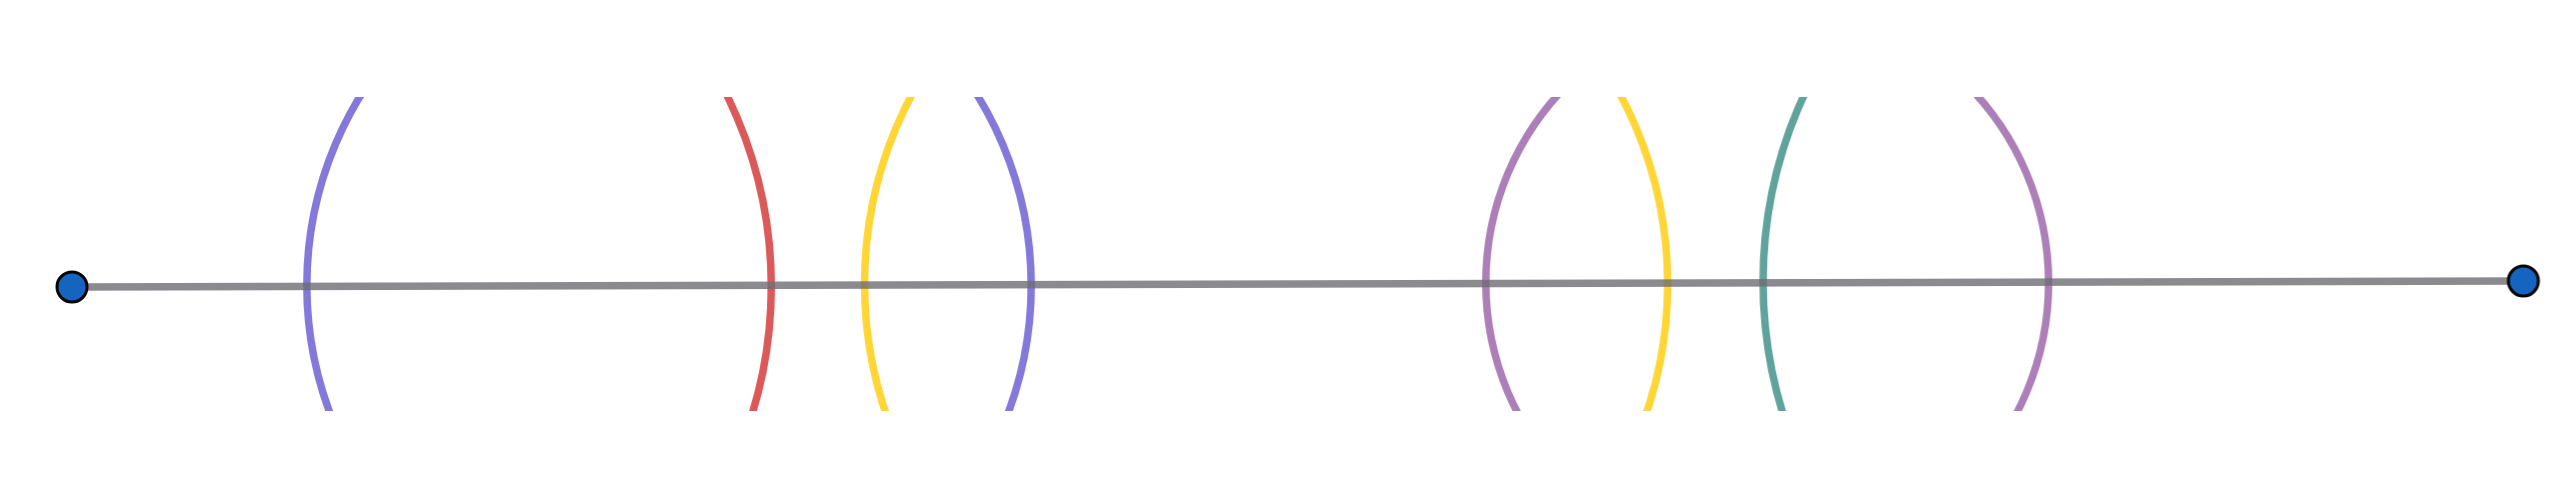
\includegraphics[width=0.8\textwidth]{pictures/wymiar_1.png}
        % \caption{wymiar}
        \label{fig:wymiar_1}
    \end{figure}
    które jest oczywiście krotności 1. 
\end{przy}
\begin{przy}
    Ewentualnie dodać przykład dla $R^2$
     \begin{figure}[H]
        \centering
        \includesvg[width=0.2\textwidth]{pictures/Refinement_on_a_planar_shape.svg}
        % \caption{zwężenie pokrycia kwadratu}
        \label{fig:wymiar_2}
    \end{figure}
    \end{przy}
\section{Twierdzenia}
Pokażemy teraz dwa twierdzenia, pierwsze mówi o tym, że zamiast szukać wpisań możemy szukać zwężeń, drugie pokazuje, że nie musimy pokazywać instnienia zwężeń dla pokryć o dowolnie dużej liczbie elementów, tylko rozważać jedynie te o ograniczonej.
\begin{twie} % 1.6.8
    Dla każdej przestrzeni normalnej $X$ NWSR:
    \begin{itemize}
        \item[(i)] wymiar pokryciowy przestrzeni $X$ jest co najwyżej $n$
        \item[(ii)] Dla każdego skończonego otwartego pokrycia $X$ możemy znaleźć otwarte wpisanie o krotności co najwyżej $n$
        \item[(iii)] Dla każdego skończonego otwartego pokrycia $X$ możemy znaleźć otwarte zwężenie o krotności co najwyżej $n$
    \end{itemize}
\end{twie}
\begin{proof}
    Zacznijmy od zauważenia, iż implikacje (i)$\Rightarrow$(ii), (ii)$\Rightarrow$(i) oraz (iii)$\Rightarrow$(i) są oczywiste, pierwsze dwie wynikają wprost z definicji wymiaru pokryciowego, w trzeciej musimy zauważyć, że każde zwężenie jest również wpisaniem. \\
    Pozostaje w takim razie pokazać implikację (ii)$\Rightarrow$(iii)\\
    Weźmy przestrzeń normalną $X$ spełniającą (ii), oraz niech $\mathcal{U}=\{U_i\}_{i=1}^k$ będzie skończonym otwartym pokryciem przestrzeni $X$. Wiemy, że istnieje $\mathcal{V}$ - otwarte wpisanie pokrycia $\mathcal{U}$ spełniające $\ord \mathcal{V}\leq n$. Teraz z tego wpisania skonstruujemy zwężenie pokrycia $\mathcal{U}$ krotności $n$.\\
    Zaczniemy od zdefiniowania przypożądkowania $i(V)$ - taki indeks z przedziału $\{1,\ldots k\}$, dla którego $V\subset U_{i(V)}$. Teraz dla każdego $i\in \{1, \ldots, k\}$ zdefiniujmy $V_i = \bigcup\{V\;|\;i=i(V)\}$. Pokażemy, że tak zdefiniowana rodzina $\tilde{\mathcal{V}}=\{V_i\}_{i=1}^k$ jest szukanym zwężeniem. \\
    Oczywiście $\forall_i\;V_i\subset U_i$ oraz $\tilde{\mathcal{V}}$ jest pokryciem przestrzeni $X$. Pozostaje więc pokazać, że $\ord \tilde{\mathcal{V}}\le n$, jednak to wynika wprost z prostej teorii zbiorów oraz $\ord\mathcal{V}\le n$ (czyli że przecięcie każdych $n+2$ parami różnych elementów $\mathcal{V}$ jest puste), co kończy dowód. 

\end{proof}

\begin{twie} %1.6.9
    Przestrzeń normalna $X$ ma wymiar pokryciowy $\dim X \leq n $ wtedy i tylko wtedy, gdy dla każdego $n+2$ elementowego otwartego pokrycia przestrzeni $X$ - $\{U_i\} _{i=1}^{n+2}$ istnieje otwarte zwężenie $ \{W_i\} _{i=1}^{n+2}$ o krotności $\ord W\le n$, spełniające $\bigcap_{i=1}^{n+2} W_i = \emptyset$.
\end{twie}
\begin{proof}
    Zauważmy, że do dowodu tego twierdzenia wystarczy pokazać, że jeżeli przestrzeń normalna $X$ ma wymiar pokryciowy większy od $n$, to jesteśmy w stanie znaleźć $\mathcal{U}=\{U_i\}_{i=1}^{n+2}$ - takie otwarte pokrycie $n+2$-elementowe, że każde jego otwarte zwężenie $\mathcal{W}=\{W_i\}_{i=1}^{n+2}$ spełnia $\bigcap\mathcal{W}\ne \emptyset$\\
    Teraz mamy $\dim X>n$, więc wiemy że możemy znaleźć takie otwarte pokrycie $\mathcal{V}=\{V_i\}_{i=1}^{k}$ przestrzeni $X$, dla którego nie istnieje otwarte zwężenie krotności $\le n$. \\
    Do tego, jeżeli $\mathcal{V}' = \{V_i'\}_{i=1}^k$ to otwarte zwężenie pokrycia $\mathcal{V}$, to spełnia ono: 
    \[V_{i_1}\cap V_{i_2} \cap \cdots \cap V_{i_m} \ne \emptyset\;\;\;\Rightarrow\;\;\;
    V'_{i_1}\cap V'_{i_2} \cap \cdots \cap V'_{i_m} \ne \emptyset\]
    Jeżeli tak nie zachodzi, to zastępujemy $\mathcal{V}$ przez $\mathcal{V'}$. Liczba różnych przecięć jest skończona, więc po skończonej liczbie podstawień ustatkujemy się (przy każdym podstawieniu eliminujemy co najmniej jedną sprzeczną implikację).\\
    Teraz, wiemy że krotność naszego pokrycia $\mathcal{V}$ spełnia $\ord\mathcal{V}>n$, więc możemy tak przeindeksować jego elementy by zachodziła własność
    \[\bigcap_{i=1}^{n+2} V_i\ne \emptyset\]
    Pokażemy, że pokrycie $\mathcal{U} = \{U_i\}_{i=1}^{n+2}$ zdefiniowane przez:
    \[U_i=V_i\;\; \mathrm{dla}\;\; i=1,2,\ldots,n+1\]
    \[U_{n+2}= \bigcup _{i=n+2}^kV_i\]
    jest szukanym pokryciem przestrzeni $X$, czyli że dla każdego otwartego zwężenia $\mathcal{W}=\{W_i\}_{i=1}^{n+2}$ pokrycia $\mathcal{U}$ zachodzi $\bigcap\mathcal{W}\ne \emptyset$.\\
    Weźmy więc dowolne zwężenie $\mathcal{W}$ pokrycia $\mathcal{U}$. Zauważmy, że
    \[\mathcal{W'}=\{W_1, W_2, \ldots, W_{n+1}, W_{n+2}\cap V_{n+2}, \ldots W_{n+2}\cap V_{k}\}  \]
    jest zwężeniem pokrycia $\mathcal{V}$. Więc
    \[\bigcap\mathcal{W} = \bigcap_{i=1}^{n+2}W_i\supset \bigcap_{i=1}^{n+1}W_i\cap (W_{n+2}\cap V_{n+2}) \ne \emptyset\]
    co kończy dowód.
\end{proof}

\begin{wnio}
    Do pokazania, że przestrzeń $X$ ma wymiar pokryciowy mniejszy równy $n$, wystarczy sprawdzać otwarte pokrycia $n+2$ elementowe.
\end{wnio}

\section{Mały i duży wymiar indukcyjny}
Tak jak wspomniane było we wstępie, poza wymiarem pokryciowym często mówimy również o dwóch inaczej zdefiniowanych wymiarach, są one jednak ze sobą powiązane.

\begin{defi}
    \emph{Małym wymiarem indukcyjnym} przestrzeni regularnej $X$ (oznaczamy $\ind  X$) nazwiemy liczbę całkowitą co najmniej $-1$ bądź $\infty$ spełniającą:
    \begin{itemize}
        \item[(MU1)] $\ind X = -1$ wtedy i tylko gdy przestrzeń $X$ jest pusta,
        \item[(MU2)] $\ind X\le n$ dla $n=0,1,\ldots$ jeżeli dla każdego punktu $x\in X$ i każdego jego otoczenia $V$ istnieje pewnien zbiór otwarty $U\subset X$ spełniający
        \[x\in U\subset V\;\;\;\mathrm{oraz}\;\;\; \ind \Fr U \le n-1\]
        \item[(MU3)] $\ind X=n$ jeżeli zachodzą nierówności $n-1<\ind X\leq n$,
        \item[(MU4)] $\ind X=\infty$, jeżeli dla każdego $n=-1,0,1,\ldots$ zachodzi $\ind X >n$
    \end{itemize}
\end{defi}
MU pochodzi tutaj od nazwisk Menger-Urysohn \cite{menger1923}, \cite{urysohn1922}. \\
Korzystając z indukcji ze względu na wymiar przestrzeni, łatwo można pokazać że jeżeli $X$ i $Y$ są homeomorficzne, to $\ind X=\ind Y$. \\
Udowodnione też zostało twierdzenie o podzbiorze:
\begin{twie}
    Dla każdego podzbioru $M$ przestrzeni regularnej $X$ spełnione jest 
    \[\ind M\le \ind X\]
\end{twie}
\begin{proof}
    odsyłam do dowodu twierdzenia 1.1.2 w \cite{engelking1995}.
\end{proof}
Przejdziemy teraz do kolejnej definicji.
\begin{defi}
    \emph{Dużym wymiarem indukcyjnym} przestrzeni normalnej $X$, (oznaczamy $\Ind X$) nazwiemy liczbę całkowitą co najmniej $-1$ bądź $\infty$ spełniającą:
    \begin{itemize}
        \item[(BČ1)] $\ind X = -1$ wtedy i tylko gdy przestrzeń $X$ jest pusta,
        \item[(BČ2)] $\ind X\le n$ dla $n=0,1,\ldots$ jeżeli dla każdego zbioru domkniętego $A$ w $X$ i każdego jego otwartego otoczenia $V$ istnieje pewnien zbiór otwarty $U\subset X$ spełniający
        \[A\subset  U\subset V\;\;\;\mathrm{oraz}\;\;\; \Ind \Fr U \le n-1\]
        \item[(BČ3)] $\ind X=n$ jeżeli zachodzą nierówności $n-1<\ind X\leq n$,
        \item[(BČ4)] $\ind X=\infty$, jeżeli dla każdego $n=-1,0,1,\ldots$ zachodzi $\ind X >n$
    \end{itemize}
\end{defi}
Skrót \emph{BČ} pochodzi tutaj od nazwisk Brouver i Čech \cite{bro1913}, \cite{cech1993}. 
Łatwo możemy pokazać, że podobnie jak dla poprzedniej definicji, dla homeomorficznych przestrzeni normalnych $X\cong Y$ zachodzi $\Ind X=\ind Y$. Oczywiście też dla każdej przestrzeni normalnej $X$ spełniona jest nierówność $\ind X\le \Ind X$, jako że wymiary pokrywają się na dziedzinie przestrzeni metrycznych ośrodkowych. 

Ważne twierdzenie, wiążące te wymiary ze sobą to:
\begin{twie}
    Dla każdej przestrzeni metrycznej ośrodkowej $X$ spełnione są równości
    \[\dim X = \ind X = \Ind X\]
\end{twie}
\begin{proof}
    Pierwsza część równości udowodniona została w (cite todo)
    druga.
\end{proof}
Mimo że na przestrzeniach metrycznych ośrodkowych te wymiary pokrywają się, w ogólności, na dużo bardziej skomplikowanych przestrzeniach zaczynają się one rozjeżdżać. Wiemy jednak, że dla przestrzeni \emph{T1} spełnione są $\ind X \le \Ind X$, a dla przestrzeni normalnych $\dim X\le \Ind X$.

% \chapter{Teoria wymiaru}
% \input{chapters/teoria_wymiaru}

\chapter{Wielościany}
% \section{podstawowe definicje}
% ewentualnie dodać definicje 
% \begin{itemize}
%     \item afinicznej niezależności
% \end{itemize}
W tej części, zdefiniujemy pojęcie wielościanu, oraz inne powiązane z nim definicje i własności.


\section{sympleksy}
\begin{defi}
    Niech punkty $p_0, p_1, \cdots, p_n$ będą afinicznie niezależne w przestrzeni $\mathbb{R}^m$. Wtedy \emph{n-sympleksem} rozpiętym na punktach $p_0, p_1, \cdots , p_n$ (oznaczmy $\Delta(p_0, p_1, \cdots , p_n)$ ) nazwiemy podzbiór punktów $p$ należących do przestrzeni $\mathbb{R}^m$ spełniających
    \[p=\lambda_0 p_0+ \lambda_1 p_1 +\cdots + \lambda_n p_n\]
    \[\sum _{i=0}^n \lambda_i = 1, \;\; \lambda _i\geq 0 \;\forall i=0,1,\ldots,n\]
    Wagi $\lambda_i, i=0,1,\ldots,n$ nazywane \emph{współrzędnymi barycentrycznymi}, są wyznaczone jednoznacznie.
    \begin{figure}[H]
        \centering
        % 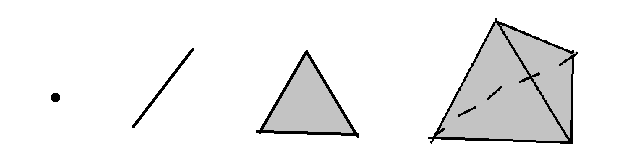
\includegraphics[width=0.8\textwidth]{pictures/sympleksy.png}
        
\begin{tikzpicture}[scale=1.2]

% ============================================
% 1. PUNKT
% ============================================
\begin{scope}[shift={(-4,0)}]
    \fill (0,0) circle[radius=3pt];
\end{scope}

% ============================================
% 2. ODCINEK
% ============================================
\begin{scope}[shift={(-2,0)}]
    \draw[thick] (0,-1) -- (0,1);
    \fill (0,-1) circle[radius=2pt];
    \fill (0,1) circle[radius=2pt];
\end{scope}

% ============================================
% 3. TRÓJKĄT
% ============================================
\begin{scope}[shift={(0,-0.5)}]
     \fill[gray!20] (0,0) -- (2,0) -- (1,1.5) -- cycle;
    \draw[thick] (0,0) -- (2,0) -- (1,1.5) -- cycle;
    \fill (0,0) circle[radius=2pt];
    \fill (2,0) circle[radius=2pt];
    \fill (1,1.5) circle[radius=2pt];
\end{scope}

% ============================================
% 4. OSTROSŁUP TRÓJKĄTNY
% ============================================
\begin{scope}[shift={(4,-0.5)}]
    \tdplotsetmaincoords{70}{120}
    \begin{scope}[tdplot_main_coords, scale=0.8]
        
        % Wierzchołki
        \coordinate (A) at (0,0,0);
        \coordinate (B) at (2,0,0);
        \coordinate (C) at (0.5,1.5,0);
        \coordinate (S) at (0.8,0.6,2.5);
        
        \fill[gray!20] (S) -- (C) -- (B) -- cycle;
        
        % Krawędzie podstawy
        \draw[thick] (B)-- (C);
        \draw[dashed] (B) -- (A);
        \draw[dashed] (C) -- (A);
        
        % Krawędzie boczne
        \draw[thick] (S) -- (C);
        \draw[thick] (S) -- (B);
        \draw[dashed] (S) -- (A);
        
        % Wierzchołki
        \fill (A) circle[radius=2pt];
        \fill (B) circle[radius=2pt];
        \fill (C) circle[radius=2pt];
        \fill (S) circle[radius=2pt];
        
    \end{scope}
\end{scope}

\end{tikzpicture}
        \caption{0,1,2,3-sympleksy w przestrzeni $\mathbb{R}^3$}
        \label{fig:sympleksy}
    \end{figure}
\end{defi}
Inna znana definicja sympleksu to $\Delta(p_0, p_1, \cdots , p_n)=conv(\{p_0, p_1, \cdots , p_n\})$, czyli najmniejszy zbiór wypukły, zawierający punkty $p_0, p_1, \cdots , p_n$. Łatwo możemy pokazać, że będzie to również zbiór zwarty w $\mathbb{R}^m$

Zauważmy, że kożystając z jednoznaczości współrzędnych barycentrycznych, wszystkie $n$-sympleksy będą wzajemnie homeomorficzne, a dodając do tego ciągłość rzutowania na współrzędne, możemy pokazać ich homeomorficzność z hiperkostką $I^n$, z czego od razu dostajemy, że wymiar pokryciowy każdego $n$-sympleksu będzie dokładnie $n$. 

Teraz wprowadzimy kilka pomocniczych definicji

\begin{defi}
    \emph{k-wymiarową ścianą} n-sympleksu rozpiętego na punktach $p_0, p_1, \ldots, p_n$ $(0\le k\le n)$ nazwiemy każdy k-sympleks rozpięty na punktach $p_{i_0}, p_{i_1},\ldots, p_{i_k}$ dla parami różnych $0\le i_j\le n$, $0\le j\le k$.\\
    0-wymiarowe ściany nazwiemy \emph{wierzchołkami}, \\
    \emph{brzegiem}, nazwiemy zbiór $S$ - zbiór wszystkich k-wymiarowych ścian,
    dopełnienie brzegu - \emph{wnętrzem}.
\end{defi}

\section{wielościany}
\begin{defi}
    \emph{Kompleksem symplicjalnym} (lub po prostu kompleksem), nazwiemy dowolną skończoną rodzinę $\mathcal{K}$ sympleksów w przestrzeni euklidesowej spełniającą:
    \begin{itemize}
        \item jeżeli sympleks $S$ należy do $\mathcal{K}$, to każda ściana $S_0$ sympleksu $S$, również należy do $\mathcal{K}$,
        \item jeżeli sympleksy $S_1, S_2$ należą do kompleksu $\mathcal{K}$, to ich przecięcie $S_1 \cap S_2$ jest puste lub jest ścianą obu sympleksów.
    \end{itemize}
    0-sympleksy w $\mathcal{K}$ nazywamy \emph{wierzchołkami}, a każdą podrodzinę $\mathcal{K}_0\subset \mathcal{K}$ która też jest kompleksem nazwiemy \emph{podkompleksem $\mathcal{K}$}.
    \begin{figure}[H]
        \centering
        % 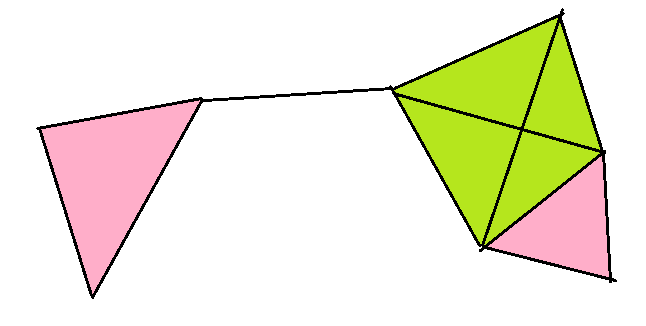
\includegraphics[width=0.8\textwidth]{pictures/kompleks.png}
        \resizebox{0.8\textwidth}{!}{%
\begin{tikzpicture}[scale=1.2]

\begin{scope}[shift={(0,0)}]
        \coordinate (A) at (-3,0);
        \coordinate (B) at (2,0);
        \coordinate (C) at (-7,-1);
        \coordinate (D) at (-5.5,-4);
        \coordinate (E) at (6,1);
        \coordinate (F) at (4,-3);
        \coordinate (G) at (7.5,-1);
        \coordinate (H) at (7,-4.5);

        \fill[gray!20] (A) -- (C) -- (D) -- cycle;
        \fill[gray!20] (F) -- (G) -- (H) -- cycle;
        \fill[gray!50] (B) -- (E) -- (G) -- (F) -- cycle;
        
        \draw[thick] (A) -- (C) -- (D) -- cycle;
        \draw[thick] (B) -- (A);
        \draw[thick] (B) -- (E) -- (G) -- (F) --cycle;
        \draw[thick] (G) -- (H) -- (F);
        \draw[thick] (E) -- (F);
        \draw[dashed] (B) -- (G);
        
        % Wierzchołki
        \fill (A) circle[radius=2pt];% node[below] {$A$};
        \fill (B) circle[radius=2pt];% node[below] {$B$};
        \fill (C) circle[radius=2pt];% node[below] {$C$};
        \fill (D) circle[radius=2pt];% node[above] {$D$};
        \fill (E) circle[radius=2pt];% node[above] {$E$};
        \fill (F) circle[radius=2pt];% node[above] {$F$};
        \fill (G) circle[radius=2pt];% node[above] {$G$};
        \fill (H) circle[radius=2pt];% node[above] {$H$};
\end{scope}

\end{tikzpicture}
}
        \caption{kompleks symplicjalny}
        \label{fig:kompl}
    \end{figure}
\end{defi}
\begin{przy}
       
% todo przykład
przykład
\end{przy}
% todo wymiar kompleksu
\begin{defi}
    Jeżeli $\mathcal{K}$ jest kompleksem symplicjalnym, to \emph{bryłą} nazwiemy zbiór punktów
    \[|\mathcal{K}|=\bigcup \{S:S\in \mathcal{K}\}\]
\end{defi}

\begin{defi}
    Każdy zbiór $W\in R^n$ dla którego istnieje kompleks symplicjalny $\mathcal{K}$ taki, że $W=|\mathcal{K}|$ 
    nazwiemy \emph{wielościanem}. $\mathcal{K}$ nazwiemy \emph{triangulacją}
\end{defi}
Przez wymiar wielościanu, uznamy wymiar największego $n$-sympleksu zawierającego się w jego triangulacji. Łatwo możemy pokazać, że tak wybrane $n$ nie zależy od wybranej triangulacji, a jedynie od samego wielościanu. Tak zdefiniowaną wartość, nazwiemy wymiarem geometrycznym wielościanu. Wynika zatem, że dla wielościanu wymiar geometryczny i pokryciowy pokrywają się. 

Warto zauważyć, że współrzędne barycentryczne można przedłużyć z sympleksów do całego wielościanu:\\ mając wielościan $K=|\mathcal{K}|$ kompleksu $\mathcal{K}$ oraz jego wierzchołki $p_0, \ldots, p_k$ każdy punkt $p\in K$ możemy reprezentować przez
\[p=\lambda_0 p_0+\cdots +\lambda_k p_k\]
dla $\lambda_0 +\cdots +\lambda_k=1$ oraz $\lambda_i\ge 0\;\;\; \forall i=0, \ldots, k$.
Oczywiście też, jeżeli $\lambda_{i_j}>0$, $j=0, \ldots, l$ to punkt $p$ musi zawierać się w $l-$sympleksie $\Delta(p_{i_0}, \ldots, p_{i_l})$. Jest to również najmniejszy (ze względu na wymiar) sympleks zawierający punkt $p$.\\
Korzystając z tak wprowadzonych współczynników, zdefiniujemy tak zwane \emph{gwiazdy}.

\begin{defi}
    Dla każdego wierzchołka $p_i$ kompleksu symplicjalnego $\mathcal{K}$, \emph{gwiazdą rozpiętą w punkcie $p_i$} nazwiemy zbiór
    \[
     \St_{\mathcal{K}}(p_i) = 
     |\mathcal{K}| \backslash \bigcup\{ S\in \mathcal{K}\;|\;p_i\not \in S\}
    \]
    \begin{figure}[H]
        \centering
        % 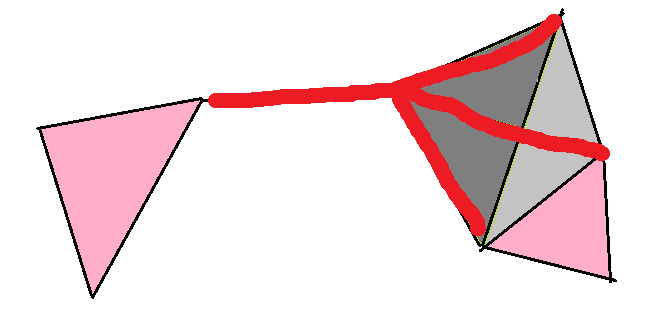
\includegraphics[width=0.8\textwidth]{pictures/gwiazda.png}
        \resizebox{0.8\textwidth}{!}{
\begin{tikzpicture}[scale=1.2]

\begin{scope}[shift={(0,0)}]
        \coordinate (A) at (-3,0);
        \coordinate (B) at (2,0);
        \coordinate (C) at (-7,-1);
        \coordinate (D) at (-5.5,-4);
        \coordinate (E) at (6,1);
        \coordinate (F) at (4,-3);
        \coordinate (G) at (7.5,-1);
        \coordinate (H) at (7,-4.5);

        \fill[gray!20] (A) -- (C) -- (D) -- cycle;
        \fill[gray!20] (F) -- (G) -- (H) -- cycle;
        \fill[gray!50] (B) -- (E) -- (G) -- (F) -- cycle;

        
        \fill[red!40] (F) -- (E) -- (B) -- cycle;
        \fill[red!20] (F) -- (G) -- (E) -- cycle;
        
        \draw[thick] (A) -- (C) -- (D) -- cycle;
        \draw[red!100][thick] (B) -- (A);
        \draw[thick] (B) -- (E) -- (G) -- (F) --cycle;
        \draw[thick] (G) -- (H) -- (F);
        \draw[thick] (E) -- (F);
        \draw[red!80][dashed] (B) -- (G);
        \draw[red!100][thick] (B) -- (E);
        \draw[red!100][thick] (B) -- (F);
        
        % Wierzchołki
        \fill (A) circle[radius=2pt];% node[below] {$A$};
        \fill[red!100] (B) circle[radius=2pt] node[above] {$p_i$};
        \fill (C) circle[radius=2pt];% node[below] {$C$};
        \fill (D) circle[radius=2pt];% node[above] {$D$};
        \fill (E) circle[radius=2pt];% node[above] {$E$};
        \fill (F) circle[radius=2pt];% node[above] {$F$};
        \fill (G) circle[radius=2pt];% node[above] {$G$};
        \fill (H) circle[radius=2pt];% node[above] {$H$};
\end{scope}

\end{tikzpicture}
}
        \caption{Gwiazda}
        \label{fig:gwiazda}
    \end{figure}
\end{defi}
Łatwo możemy pokazać, że 
$
\St_{\mathcal{K}}(p_i) = 
     \{ p\in |\mathcal{K}|\;:\;\lambda_i>0\}
$,
z czego wynika, że gwiazdy są otwartymi podzbiorami wielościanu $|\mathcal{K}|$

Mimo, że technicznie kompleksy symplicjalne i wielościany są innymi obiektami, w dalszej części pracy będziemy je utożsamiać ze sobą, w części której nam jest to potrzebne używać własności kompleksu symplicjalnego, w innej odpowiadającemu mu wielościanu.


\chapter{Nerw}
\section{położenie ogólne}
\begin{defi}
    Powiemy, że punkty $p_1, p_2, \ldots , p_k \in \mathbb{R}^m$ są w \emph{położeniu ogólnym}, jeżeli dla każdego ciągu $l+1$ liczb naturalnych $0< i_0<i_1<\cdots<i_l<k$, $l<m$, punkty $p_{i_0}, p_{i_1},\ldots, p_{i_l}$ tworzą układ afinicznie niezależny.
\end{defi}
\begin{przy}
    Zauważmy, że na płaszczyźnie $\mathbb{R}^2$, zbiór punktów z których każde dowolnie wybrane 3 nie są współliniowe będzie w położeniu ogólnym.
    \begin{figure}[H]
        \centering
        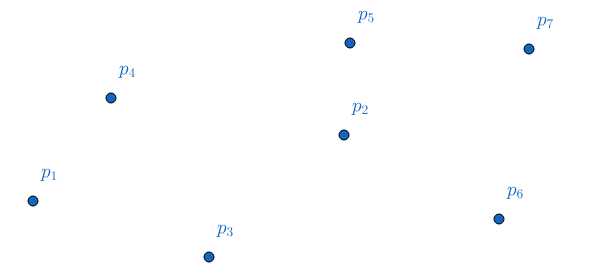
\includegraphics[width=0.5\textwidth]{pictures/polozenie_ogolne.png}
        \caption{Układ w położeniu ogólnym}
        \label{fig:polozenie_ogolne}
    \end{figure}
    Na rysunku \ref{fig:polozenie_ogolne} punkty $p_1, \ldots, p_7$ twożą oczywiście taki układ.
\end{przy}

\begin{twie}
    \label{twie:1_10_2}
    Dla ciągu punktów $q_1, q_2, \ldots, q_k\in \mathbb{R}^m$ i dla każdej liczby $\alpha>0$ istnieją punkty $p_1, p_2, \ldots , p_k\in \mathbb{R}^m$ w położeniu ogólnym, spełniające $\rho (p_i, q_i)<\alpha$$ \forall i=1,2,\ldots,k$.\\
    Ponadto, jeżeli układ $r_1, r_2, \ldots , r_l\in R^m$ jest w położeniu ogólnym, to możemy tak wybrać punkty $p_1, p_2, \ldots , p_k\in R^m$ 
    by $r_1, r_2, \ldots , r_l, p_1, p_2, \ldots , p_k$ również tworzyły układ w położeniu ogólnym.
\end{twie}
\begin{proof}
    Wynika wprost z indukcji:\\
    $p_1$ zdefiniujemy po prostu jako $q_1$, teraz pokażemy krok indukcjyjny.
    Załóżmy że punkty $p_1, \ldots, p_{j-1}$ są dobrze zdefiniowane, czyli tworzą układ w położeniu ogólnym oraz spełniają $\rho(p_i, q_i)<\alpha$ dla $i=1, \ldots, j-1$.\\
    Zauważmy teraz, że każdy co najwyżej $m-1$ elementowy podzbiór punktów $p_1, \ldots, p_{j-1}$ jest afinicznie niezależny, oraz że będą one rozpinały przestrzeń afiniczną wymiaru co najwyżej $m-1$. Czyli jest to zbiór nigdzie gęsty w $\mathbb{R}^m$. Ponieważ wszystkich takich podzbiorów jest skończenie wiele, to suma przestrzeni afinicznych rozpiętych na nich również będzie nigdzie gęsta. Wynika z tego, jesteśmy w stanie znaleźć taki punkt $p_j$ poza tym zbiorem, który będzie spełniał $\rho (p_j, q_j)<\alpha$.\\
    \\
    Dowód dla drugiej części twierdzenia jest analogiczny. 
    \begin{figure}[H]
        \centering
        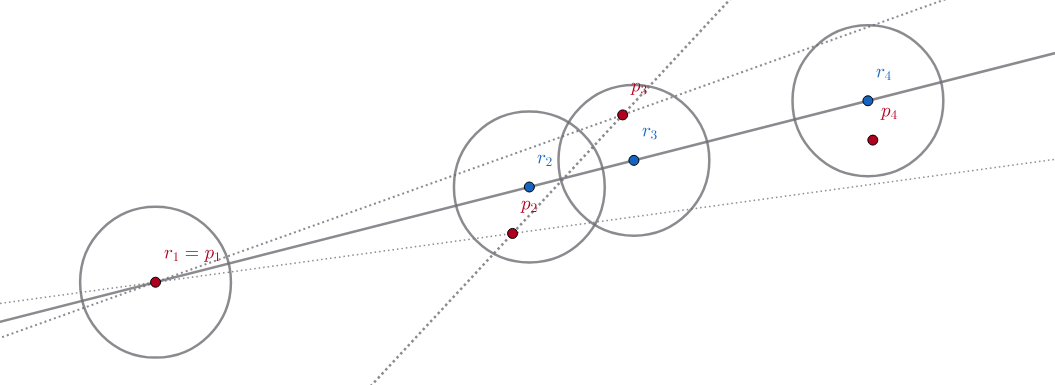
\includegraphics[width=0.8\textwidth]{pictures/polo_tw_konstrukcja.png}
        \caption{Szkic konstrukcji}
        \label{fig:szkic}
    \end{figure}
\end{proof}


\section{Nerw}

\begin{defi}
    \cite{alex1927} 
    Niech $\mathcal{U} = \{U_i\}_{i=1}^k$ będzie skończonym otwartym pokryciem przestrzeni topologicznej $X$.
    \emph{Nerwem} pokrycia $\mathcal{U}$ nazwiemy dowolny kompleks symplicjalny $\mathcal{N(U)}$, 
    którego wierzchołki możemy ustawić w ciąg $p_1, p_2, \ldots, p_k$ w taki sposób, że
    \[p_{i_0}p_{i_1} \ldots p_{i_m}\in \mathcal{N(U)} \Leftrightarrow U_{i_0}\cap U_{i_1}\cap \cdots \cap U_{i_m}\neq \emptyset \]
\end{defi}
\begin{przy}
    \begin{figure}[H]
        \centering
        % 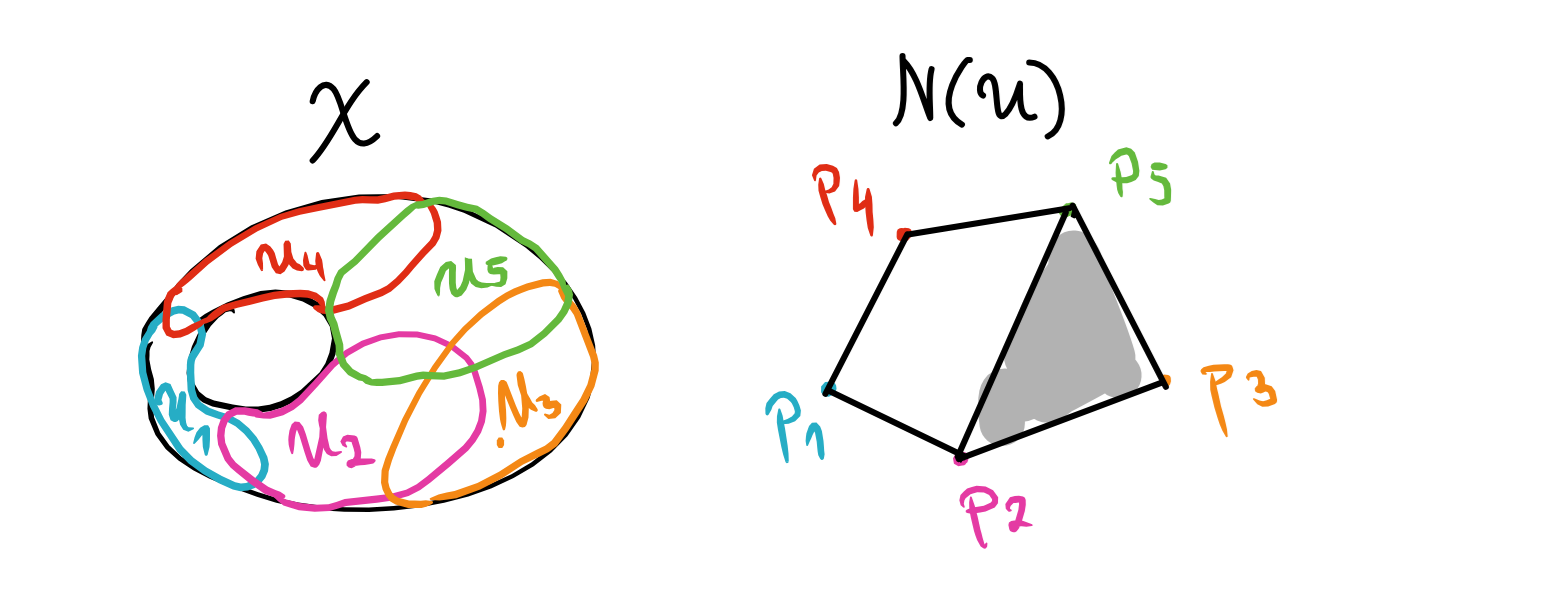
\includegraphics[width=0.8\textwidth]{pictures/nerw_2.png}
        \resizebox{0.7\textwidth}{!}{%
\definecolor{colCyan}{RGB}{0, 168, 204}
\definecolor{colRed}{RGB}{220, 50, 32}
\definecolor{colGreen}{RGB}{92, 172, 45}
\definecolor{colPink}{RGB}{225, 60, 140}
\definecolor{colOrange}{RGB}{245, 130, 32}
\definecolor{colGray}{RGB}{180, 180, 180}

\centering

\begin{tikzpicture}[line cap=round, line join=round]

% ================= Lewy diagram: Przestrzeń X (zmniejszony) =================
\begin{scope}[local bounding box=left, scale=0.45]
  % Tytuł
  \node at (3.5, 7) {\Huge $\mathcal{X}$};

  % Współrzędne P
  {
  \coordinate (P1) at (-4, 0);
  \coordinate (P2) at (-3.1, 2);
  \coordinate (P3) at (-2, 3);
  \coordinate (P4) at (0.0, 3.8);
  \coordinate (P5) at (2, 4.2);
  \coordinate (P6) at (3.5, 4.3);
  \coordinate (P7) at (5.3, 4.2);
  \coordinate (P8) at (7, 4);
  \coordinate (P9) at (9, 3);
  \coordinate (P10) at (10, 1);
  \coordinate (P11) at (10.1, -0.6);
  \coordinate (P12) at (10, -2);
  \coordinate (P13) at (9.5, -3.2);
  \coordinate (P14) at (8.7, -4.4);
  \coordinate (P15) at (7,-5);
  \coordinate (P16) at (5, -5.3);
  \coordinate (P17) at (3, -5.3);
  \coordinate (P18) at (1, -5);
  \coordinate (P19) at (-0.7, -4.4);
  \coordinate (P20) at (-2, -3.8);
  \coordinate (P21) at (-3, -3);
  \coordinate (P22) at (-3.8, -1.6);
  \coordinate (P23) at (-3.6, 1.2);

  % Współrzędne R
  \coordinate (R1) at (-0.8, 0);
  \coordinate (R2) at (-0.2, 1.4);
  \coordinate (R3) at (1, 2);
  \coordinate (R4) at (2,2.1);
  \coordinate (R5) at (2.8, 1.9);
  \coordinate (R6) at (3.5,1.5);
  \coordinate (R7) at (4,1);
  \coordinate (R8) at (4.2,0.3);
  \coordinate (R9) at (4,-0.6);
  \coordinate (R10) at (3,-1.6);
  \coordinate (R11) at (1.7, -1.8);
  \coordinate (R12) at (0.5,-1.5);
  \coordinate (R13) at (-0.4, -0.8);
  \coordinate (R14) at (-0.7, 0.8);

  % Współrzędne U
  \coordinate (U1) at (-1.2, 2.9);
  \coordinate (U2) at (-1.6, 1);
  \coordinate (U3) at (-0.8, -1.8);
  \coordinate (U4) at (1.6, -3.8);
  \coordinate (U5) at (5.2, -0.4);
  \coordinate (U6) at (3.6, 2.6);
  \coordinate (U7) at (6.4, 3.6);
  \coordinate (U8) at (4.8, 1.5);
  \coordinate (U9) at (1,-2);
  \coordinate (U10) at (0, -4.4);
  \coordinate (U11) at (-0.1, 2.1);
  \coordinate (U12) at (-2.6, 2.4);
  \coordinate (U13) at (-2.7, 1);
  \coordinate (U14) at (-1.2, -3);
  \coordinate (U15) at (7.6, -3.4);
  \coordinate (U16) at (4.2, -1.4);
  \coordinate (U17) at (9.1, -1.4);
  \coordinate (U18) at (4.2, 3.7);
  \coordinate (U19) at (5.1, -3.8);
  \coordinate (U20) at (7.8, 1);
  \coordinate (U21) at (7.6, -0.7);

  % Rysowanie punktów P, R, U
  % \foreach \p in {P1,...,P23} \fill[black!100] (\p) circle (3pt);
  % \foreach \p in {R1,...,R14} \fill[black!100] (\p) circle (3pt);
  % \foreach \p in {U1,...,U21} \fill[black!100] (\p) circle (3pt);

  % % Etykiety P
  % \foreach \i in {1,...,23} \node[colRed, above left=2pt] at (P\i) {\Large $P_{\i}$};

  % % Etykiety R
  % \foreach \i in {1,...,14} \node[colGreen, above left=2pt] at (R\i) {\Large $R_{\i}$};

  % % Etykiety U (czarne)
  % \foreach \i in {1,...,21} \node[black!100, above left=2pt] at (U\i) {\Large $U_{\i}$};
  }

  % Zewnętrzna granica
  \draw[line width=5pt, black!100] plot [smooth cycle, tension=0.6] coordinates {
    (P1) (P23) (P2) (P3) (P4) (P5) (P6) (P7) (P8) (P9) 
    (P10) (P11) (P12) (P13) (P14) 
    (P15) (P16) (P17) (P18) (P19) 
    (P20) (P21) (P22) 
  };

  % Wewnętrzna granica R
  \draw[line width=5pt, black!100] plot [smooth cycle, tension=0.6] coordinates {
    (R1) (R14) (R2) (R3) (R4) (R5) 
    (R6) (R7) (R8) (R9)  
    (R10) (R11) (R12) (R13) 
  };

  % Kształty U
  \draw[line width=4pt, colCyan] plot [smooth cycle, tension=0.6] coordinates {
    (P1) (P23) (P2) (U12) 
    (U1) (U11) (R2) (R14) (R1) 
    (R13) (U9) (U4) (U10) (P20) (P21) (P22) 
  };

  \draw[line width=4pt, colRed] plot [smooth cycle, tension=0.6] coordinates {
    (U2) (U13) (P2) (P3) (P4) 
    (P5) (P6) (P7) (U7) 
    (U8) (R6) (R5) 
    (R4) (R3) (R2) 
  };

  \draw[line width=4pt, colPink] plot [smooth cycle, tension=0.6] coordinates {
    (U3) (R12) (R11) (R10) 
    (R9) (U5) (U21) (U15) (P15) 
    (P16) (P17) (P18) (P19) 
    (U14)
  };

  \draw[line width=4pt, colGreen] plot [smooth cycle, tension=0.6] coordinates {
    (R7) (R6) (U6) (U18) (P7) 
    (P8) (P9) (P10) (U17)
    (U16) (R9) (R8) 
  };

  \draw[line width=4pt, colOrange] plot [smooth cycle, tension=0.6] coordinates {
    (U19) (U20) (P10) (P11) 
    (P12) (P13) (P14) 
    (P15) 
  };

  % Duże etykiety U
  \node[colCyan] at (-2,-0.5) { \fontsize{17}{48}\selectfont $U_1$ };
  \node[colPink] at (3.5,-3.2) { \fontsize{17}{48}\selectfont $U_2$ };
  \node[colOrange] at (8.7,-2.5) { \fontsize{17}{48}\selectfont $U_3$ };
  \node[colRed] at (1.7,3.1) { \fontsize{17}{48}\selectfont $U_4$ };
  \node[colGreen] at (6.3,1.2) { \fontsize{17}{48}\selectfont $U_5$ };
\end{scope}

% ================= Prawy diagram: Nerw N(u) (oryginalny rozmiar) =================
\begin{scope}[local bounding box=right, shift={($(left.east)+(2.5cm,-0.2)$)}]
  % Tytuł
  \node at (1.5, 2.7) {\Huge $\mathcal{N(U)}$};

  % Współrzędne wierzchołków
  \coordinate (N1) at (-0.5, -1.3);
  \coordinate (N4) at (1.5, 1.3);
  \coordinate (N5) at (4, 1.7);
  \coordinate (N2) at (2, -2.3);
  \coordinate (N3) at (5.2, -0.6);

  % Zacieniony 2-sympleks
  \fill[colGray] (N2) -- (N5) -- (N3) -- cycle;

  % Krawędzie kompleksu
  \draw[line width=3pt, black] (N1) -- (N4) -- (N5) -- (N3) -- (N2) -- cycle;
  \draw[line width=3pt, black] (N2) -- (N5);

  % Wierzchołki
  \fill[colCyan] (N1) circle (5pt);
  \fill[colRed] (N4) circle (5pt);
  \fill[colGreen] (N5) circle (5pt);
  \fill[colPink] (N2) circle (5pt);
  \fill[colOrange] (N3) circle (5pt);

  % Etykiety wierzchołków
  \node[colCyan, below left=2pt] at (N1) {\fontsize{17}{48}\selectfont $P_1$};
  \node[colRed, above left=2pt] at (N4) {\fontsize{17}{48}\selectfont  $P_4$};
  \node[colGreen, above right=2pt] at (N5) {\fontsize{17}{48}\selectfont $P_5$};
  \node[colPink, below=4pt] at (N2) {\fontsize{17}{48}\selectfont  $P_2$};
  \node[colOrange, right=4pt] at (N3) {\fontsize{17}{48}\selectfont  $P_3$};
\end{scope}

\end{tikzpicture}
}
        \caption{nerw}
        \label{fig:nerw_2}
    \end{figure}
    dodać jakiś opis
\end{przy}
\section{twierdzenie o zanużeniu w $R^{2n+1}$}

\begin{twie}
    Niech $\mathcal{U}=\{U_i\}_{i=1}^k$ będzie skończonym otwartym pokryciem przestrzeni topologicznej $X$. Jeżeli krotność pokrycia $\mathcal{U}$ jest conajwyżej $n$, to nerw pokrycia $\mathcal{N(U)}$ możemy zrealizować w $\mathbb{R}^{2n+1}$. \\
    Ponadto, mając:
    \begin{itemize}
        \item $H$ - n-wymiarową podprzestrzeń afiniczną  $R^{2n+1}$,
        \item punkty $q_1, \ldots, q_k\in R^{2n+1}$,
        \item liczbę $\alpha>0$
    \end{itemize} 
    możemy wybrać nerw $\mathcal{N(U)}$ w taki sposób, by $\mathcal{N(U)}$ nie przecinał podprzestrzeni $H$, oraz by $p_1, \ldots, p_k$ wierzchołki nerwu $\mathcal{N(U)}$ spełniały $\rho(p_i, q_i)<\alpha$ dla $i=1,2,\ldots, k$
\end{twie}
\begin{proof}
    Możemy łatwo zauważyć, że druga część twierdzenia jest rozszerzeniem pierwszej, możemy się więc skupić na udowodnieniu tylko drugiej części.\\
    Niech $r_1, \ldots, r_{n+1}\in R^{2n+1}$ afinicznie niezależne rozpinające $H$.
    Z twierdzenia \ref{twie:1_10_2} wiemy, że możemy tak wybrać punkty $p_1, \ldots, p_k\in \mathbb{R}^{2n+1}$ by punkty $r_1, \ldots, r_{n+1}, p_1,\ldots, p_k $ były w położeniu ogólnym. \\
    Z tego, że $\ord \mathcal{U}\le n$ wiemy, że dla każdego ciągu $l+1$ indeksów $0\le i_0< \cdots < i_l\le k$ takich że $U_{i_0}\cap\cdots \cap U_{i_l}\ne \emptyset$, to $l\le n<2n+1$, czyli punkty odpowiadające tym indeksom: $p_{i_0},\ldots p_{i_l}$ tworzą układ afinicznie niezależny oraz że sympleks na nich zbudowany jest dobrze zdefiniowany. \\
    Teraz niech $\mathcal{K}$ będzie rodziną sympleksów zdefiniowanych w ten sposób. Teraz pozostaje pokazć, że tak zdefiniowana rodzina jest nerwem $\mathcal{N(U)}$ oraz że $\mathcal{N(U)}\cap H=\emptyset$.\\
    Zauważmy, że do pokazania że $\mathcal{K}$ jest nerwem, jedyne co trzeba pokazać to że $\mathcal{K}$ jest kompleksem symplicjalnym, czyli że 
    \begin{enumerate}
        \item dla każdego sympleksu $S\in \mathcal{K}$ każda jego ściana $S'$ również spełnia $S'\in \mathcal{K}$
        \item dla każdych $S_1, S_2\in \mathcal{K}$, jeżeli $S_1\cap S_2\ne \emptyset$ to $S_1\cap S_2$ musi być ścianą obu.
    \end{enumerate}
    dowód 1:\\
    Zauważmy, że skoro sympleks w $S$ oparty na wierzchołkach $p_{i_0}, \ldots, p_{i_l}$ jest w $\mathcal{K}$, to $U_{i_0}\cap\cdots\cap U_{i_l}\ne \emptyset$. Za tym od razu idzie że przecięcie każdego podzbioru $\{ U_{i_0}, \ldots, U_{i_l}\}$ musi również być niepuste, tak więc każda ściana $S$ również będzie należała do $\mathcal{K}$.
    \\
    dowód 2:\\
    Weźmy $S_1, S_2\in \mathcal{K}$, $S_1$ oparty na $p_{i_0}, \ldots, p_{i_l}$, $S_2$ oparty na $p_{j_0}, \ldots, p_{j_m}$, $l, m\le n$.\\
    Załóżmy, że sympleksy oparte są na dokładnie $0\le a\le \min(l+1, m+1)$ takich samych wierzchołkach. Możemy w takim razie tak je przeindeksować, by spełnione było:
    \[p_{i_s}=p_{j_s} \;\; \mathrm{dla} \;\;s=0,1,\ldots, a-1\]
    \[p_{i_a}, \ldots, p_{i_l}, p_{j_a},\ldots,  p_{j_m}\;\; \mathrm{parami\;\;różne}\]
    Weźmy dowolny punkt $p$ należący do przecięcia $S_1\cap S_2$. Zauważmy że skoro $p\in S_1$, to możemy przedstawić punkt $p$ jako:
    \[p=\sum _{s=0}^l \lambda_sp_{i_s}, \;\; \sum_{s=0}^l\lambda_s=1,
    \lambda_s\ge 0\forall_{s=0,1, \ldots, l} \]
    podobnie z $p\in S_2$ dostajemy:
    \[p=\sum _{t=0}^m \lambda'_tp_{i_t}, \;\; \sum_{t=0}^m\lambda'_t=1,
    \lambda'_t\ge 0\forall_{t=0,1, \ldots, m} \]
    Dostajemy w takim razie układ równań:
    \[\sum _{s=0}^l \lambda_sp_{i_s}- \sum _{t=0}^m \lambda'_tp_{i_t} = 
    0\]
    \[\sum _{s=0}^l \lambda_s - \sum _{t=0}^m \lambda'_t = 0\]
    Pierwsze równanie możemy uprościć do postaci:
    \[
    \sum _{s=0}^a (\lambda_s-\lambda'_s)p_{i_s} +
    \sum _{s=a}^l \lambda_sp_{i_s}- \sum _{t=a}^m \lambda'_tp_{i_t} = 
    0\]
    Zauważmy, że skoro $l, m\le n$, czyli $2+m+l\le 2n+2$, to punkty 
    $p_{i_0}, \ldots, p_{i_l},p_{j_a}\ldots ,p_{j_m}$ będą tworzyły układ afinicznie niezależny, z czego wynika że wszystkie wpółczynniki w powyższym równianiu muszą być równe 0, za czym idzie:
    \[\lambda_s=\lambda'_s,  \;\;\mathrm{dla}\;\;s=0,\ldots, a-1 \]
    \[\lambda_s = 0, \;\;\mathrm{dla}\;\;s=a, \ldots,l\]
    \[\lambda'_s=0,  \;\;\mathrm{dla}\;\;\;s=a,\ldots, m\]
    W takim razie punkt $p$ możemy rozpisać jako
    \[p=\sum_{s=0}^{a-1}\lambda_sp_{i_s}=\sum_{s=0}^{a-1}\lambda'_sp_{j_s}\]
    czyli punkt $p$ należy również do sympleksu opartego na $p_{i_0}, \ldots, p_{i_{a-1}}$, który jest ścianą obu sympleksów $S_1, S_2$, co kończy dowód.
    Wynika z tego, że $\mathcal{K}$ faktycznie jest nerwem pokrycia $\mathcal{U}$.\\
    Do skończenia dowodu twierdzenia wystarczy pokazać, że $H\cap \mathcal{K}=\emptyset$, jest to jednak analogiczne do powyższego.
\end{proof}

\chapter{Twierdzenie o $\varepsilon$-przekształceniach}
\section{Cel pracy}
W tym rozdziale przedstawimy twierdzenie które jest celem całej pracy, czyli twierdzenie o $\varepsilon$-przekształceniach. 
\begin{twie}
    \label{twie:o_prz}
    Zwarta przestrzeń metryczna $X$ ma wymiar pokryciowy co najwyżej $n$ wtedy i tylko wtedy, 
    gdy dla każdego $\varepsilon >0$ istnieje $\varepsilon$-przekształcenie $X$ w wielościan wymiaru co najwyżej $n$.
\end{twie}
Dla ułatwienia, dowodzić je będziemy równolegle z bardzo podobnym twierdzeniem, o $\mathcal{U}$-mapach. 
\begin{twie}
    \label{twie:o_map}
    Zwarta przestrzeń metryczna $X$ ma wymiar pokryciowy co najwyżej $n$ wtedy i tylko wtedy, gdy dla każdego skończonego otwartego pokrycia $\mathcal{U}$ przestrzeni $X$ istnieje $\mathcal{U}$-mapa $X$ w wielościan wymiaru co najwyżej $n$.
\end{twie}


\section{$\varepsilon$-przekształcenie}
Zacznijmy od wprowadzenia definicji $\varepsilon$-przekształcenia oraz $\mathcal{U}$-mapy.
\begin{defi} % 1.10.9
    Niech $\varepsilon>0$, oraz niech $f:X\rightarrow Y$ ciągłe przekształcenie przestrzeni metrycznej $X$ w przestrzeń topologiczną $Y$. 
    Wtedy, powiemy że $f$ jest \emph{$\varepsilon$-przekształceniem}, jeżeli dla każdego punktu w $Y$ średnica przeciwobrazu w tym punkcie jest mniejsza od $\varepsilon$, czyli  $\forall y\in Y \; \diam (f^{-1}(y))<\varepsilon$.
\end{defi}
\begin{przy}
    Weźmy ciąg funkcji ciągłych $f_n:[0,1]\rightarrow[0,1]$ dla $n\ge 2$ z odcinka $[0,1]$ w ten sam odcinek, zdefiniowanych
    \[
    f_n(x) =
    \begin{cases}
        0,                            & x \le \frac{1}{n+1},\\
        \frac{n+1}{n-1}(x-\frac{1}{n+1}), & x \in (\frac{1}{n+1}, \frac{n}{n+1}), \\
        1,                            & x\ge \frac{n}{n+1}.\\
    \end{cases}
    \]
    \begin{figure}[H]
        \centering
        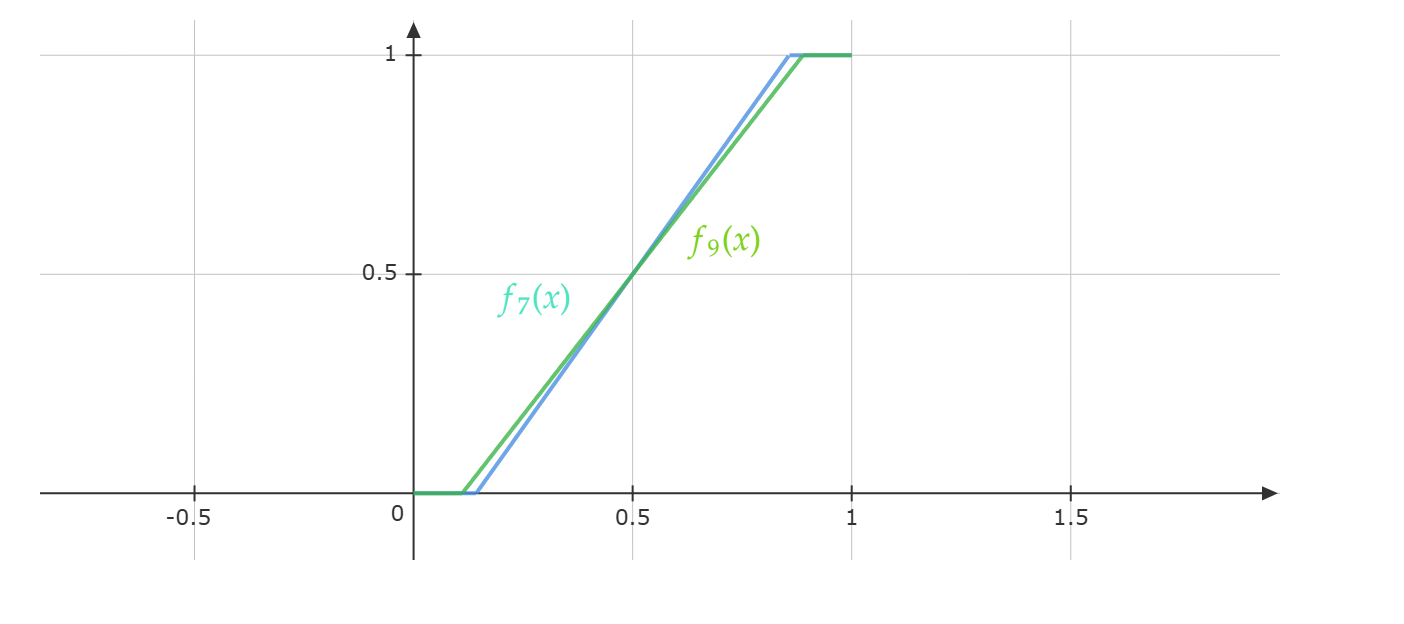
\includegraphics[width=0.8\textwidth]{pictures/eps_funkcja_przyklad.png}
        \caption{$\varepsilon$-przekształcenie}
        \label{fig:eps_2}
    \end{figure}
    Łatwo możemy sprawdzić, że tak zdefiniowane funkcje $f_n$ są odpowiednio $\frac{1}{n}$-przekształceniami (rysunek \ref{fig:eps_2}).
\end{przy}

\begin{defi} % 1.10.8
    Niech $\epsilon$ będzie otwartym pokryciem przestrzeni $X$, oraz niech $f:X\rightarrow Y$ niech będzie ciągłym przekształceniem przestrzeni $X$ w przestrzeń topologiczną $Y$.\\
    Powiemy że $f$ jest \emph{$\mathcal{U}$-mapą}, jeżeli istnieje $\mathcal{V}$ takie  otwarte pokrycie $Y$, że przeciwobraz $f^{-1}(\mathcal{V})$ jest wpisaniem pokrycia $\mathcal{U}$.
\end{defi}

\begin{przy}
    Dla $n\ge 3$, weźmy pokrycie odcinka $(0,1)=I$ 
    \[U=\{(\frac{i-1}{n}, \frac{i+1}{n})\:| \; i=1, \ldots, n-1\}.\]
    Rozpatrzmy otwarty kwadrat $(0,1)\times (0,1)$ i jego dwa pokrycia
    \[U_1 = U\times I\;\;\;\mathrm{oraz}\;\;\; U_2 = I\times U.\]
    Wtedy rzutowanie na pierwszą współrzędną $\pi_1:I^2\rightarrow I$, $\pi_1(x_1,x_2)=x_1$ będzie oczywiście $U_1$-mapą, ale nie będzie $U_2$-mapą. 
\end{przy}

Teraz pokażemy twierdzenie, które pokazuje nam zależność między tymi dwoma definicjami.


\begin{twie}
    \label{twie:map_a_prze}
    Niech $X$ będzie zwartą przestrzenią metryczną, wtedy dla każdego otwartego pokrycia $\mathcal{U}$ przestrzeni $X$, istnieje taka liczba dodatnia $\varepsilon>0$, że każde $\varepsilon$-przekształcenie w przestrzeń Hausdorffa jest też $\mathcal{U}$-mapą.
\end{twie}
\begin{proof}
    Weźmy dowolne otwarte pokrycie $\mathcal{U}$ przestrzeni $X$. Teraz niech $\varepsilon>0$ będzie liczbą Lebesgue'a pokrycia $\mathcal{U}$ - czyli taką wielkością, że dla każdego podzbioru $A\subset X$, jeżeli średnica $\delta(A)$ jest mniejsza od $\varepsilon$, to $A$ zawiera się w którymś elemencie pokrycia $\mathcal{U}$.\\
    Weźmy teraz dowolne $\varepsilon$-przekształcenie $f:X\rightarrow Y$, gdzie $Y$ to przestrzeń Hausdorffa. Pokażemy, że musi ono być również $\mathcal{U}$-mapą.\\
    Zauważmy, że dla każdego elementu $y\in Y$ możemy znaleźć taki element pokrycia $U_y\in \mathcal{U}$, dla którego $f^{-1}(y)\subset U_y$. Z tego że funkcja $f$ jest przekształceniem ciągłym z przestrzeni zwartej w przestrzeń Hausdorffa wiemy, że jest zamknięta na zbiory zamknięte, więc zbiór
    \[V_y = Y\backslash f(X\backslash U_y)\]
    jest oczywiście otwarty. Łatwo możemy sprawdzić, że zachodzi $y\in V_y$, oraz że $f^{-1}(V_y)\subset U_y$. \\
    W takim razie zbiór $\mathcal{V} = \{V_y\}_{y\in Y}$ będzie pokryciem przestrzeni $Y$ spełniającym $f^{-1}(V)$ jest wpisaniem $\mathcal{U}$, co kończy dowód.
\end{proof}
Udowodnimy teraz dwa twierdzenia pomocnicze. 
\begin{twie} % 1.10.11
    \label{twie:1_10_11}
    Jeżeli dla każdego otwartego skończonego pokrycia $\mathcal{U}$ przestrzeni normalnej $X$ istnieje $\mathcal{U}$-mapa w przestrzeń zwartą $Y$ wymiaru co najwyżej $n$, to $\dim X\le n$.
\end{twie}  
\begin{proof}
    Weźmy dowolne otwarte skończone pokrycie $\mathcal{U}$ przestrzeni $X$, oraz niech $f:X\rightarrow Y$ będzie $\mathcal{U}$-mapą w przestrzeń $Y$, $\dim Y\le n$.\\
    Niech $\mathcal{V}$ będzie takim otwartym pokryciem $Y$, że $f^{-1}(\mathcal{V})$ jest wpisaniem $\mathcal{U}$. Teraz skoro $Y$ jest zwarte, to $\mathcal{V}$ ma skończone otwarte wpisanie $\mathcal{V'}$, a korzystając z $\dim Y\le n$ wiemy, że dla $\mathcal{V'}$ możemy znaleźć otwarte wpisanie $\mathcal{W}$, które spełnia $\ord \mathcal{W\le }n$. \\
    Zauważmy teraz, że $f^-1(\mathcal{W})$ też jest skończonym otwartym pokryciem $X$, które jest wpisane w $\mathcal{U}$ i spełnia $\ord f^{-1}(\mathcal{W})\le n$, skąd wynika $\dim X \le n$, co kończy dowód.
\end{proof}

\begin{twie} % 1.10.12
    \label{twie:1_10_12}
    Jeżeli dla każdej liczby $\varepsilon>0$ istnieje $\varepsilon$-przekształcenie zwartej przestrzeni metrycznej $X$ w zwartą przestrzeń $Y$ wymiaru co najwyżej $n$, to $\dim X\le n$.
\end{twie}
\begin{proof}
    Zauważmy, że dowód tego twierdzenia wynika wprost z twierdzeń \ref{twie:1_10_11} oraz \ref{twie:map_a_prze}: \\
    weźmy $\mathcal{U}$-dowolne otwarte pokrycie przestrzeni $X$ i jako $\varepsilon>0$ weźmy liczbę Lebesgue'a tego pokrycia. Teraz wiemy, że możemy znaleźć $\varepsilon$-przekształcenie $f:X\rightarrow Y$ które będzie też $\mathcal{U}$-mapą, więc $\dim X\le n$.
\end{proof}

Zauważmy, że twierdzenia \ref{twie:1_10_12} oraz \ref{twie:1_10_11} są tak naprawdę implikacjami w jedną stronę twierdzeń \ref{twie:o_prz} oraz \ref{twie:o_map}, jeżeli lekko zmodyfikujemy ich treści i zamienimy dowolną przestrzeń zwartą $Y$ wymiaru $\dim Y \le n$ w wielościan wymiaru $n$, dowód będzie przebiegał bardzo podobnie. \\
W takim razie, do dokończenia dowodów, jedyne co zostaje nam pokazać, to że zawsze jesteśmy w stanie takie przekształcenia znaleźć.

\section{Funkcja $\kappa$-kuratowskiego}
\begin{defi}
    Niech $\mathcal{U} = \{U_i \} _{i=1}^k$ będzie skończonym otwartym pokryciem przestrzeni topologicznej $X$ oraz niech $p_1, p_2, \ldots, p_k \in \mathbb{R}^m$ Bedzie ciągiem punktów.\\
    Ciągłe przekształcenie z przestrzeni $X$ w $\mathbb{R}^m$ $\kappa :X\rightarrow R^m$ zdefiniujmy jako
    \[\kappa(x) = \kappa_1(x)p_1+\kappa_2(x)p_2+\cdots+\kappa_k(x)p_k ,\]
    gdzie 
    \[\kappa_i(x) = \frac{\rho(x, X\backslash U_i)}{\sum _{j=1}^k\rho(x, X\backslash U_j)}.\]
    Taką funkcję nazwiemy funkcją \emph{$\kappa$-Kuratowskiego}.
    \cite{kuratowski1933}
\end{defi}
Zauważmy, że w tej definicji może zdarzyć się, że element pokrycia będzie równy całej przestrzeni $X$, czyli $U_i=X$, wtedy we wzorze pojawi się odległość punktu od zbioru pustego. By uniknąć tego problemu, skorzystamy z definicji funkcji $\rho$ zdefiniowanej w \cite{engelking1989}, dla której przyjmujemy $\rho(x, \emptyset)=1$.\\
Zwróćmy uwagę na to, że tak zdefiniowana funkcja jest dobrze określona, jako że jeżeli $x\in X$ należy do $U_i$, to $\rho(x, X\backslash U_i)>0$, za czym idzie 
$\forall x\in X\;\;\sum _{j=1}^k\rho(x, X\backslash U_j)>0$, ponieważ $\mathcal{U}$ jest pokryciem.\\ 
Własnością na którą warto zwrócić uwagę, jest to dla każdego $x\in X$ zachodzi $\sum_{i=1}^{k}\kappa_i(x)=1$, oraz oczywiście wszystkie $\kappa_i(x)\ge 0$.\\
Warto również pokazać, że przekształcenie $\kappa$ rzeczywiście jest ciągłe. To wynika jednak wprost z ciągłości funkcji $\rho(\cdot, A)$ dla ustalonego zbioru $A$, oraz oczywiście z tego, że złożenie funkcji ciągłych również jest funkcją ciągłą.\\

Udowodnimy teraz dwa twierdzenia, pierwsze mówi o przybliżaniu ciągłych przekształceń funkcjami $\kappa$-Kuratowskiego, a drugie jest o własnościach tej funkcji.

\begin{twie} % 1.10.6
    Niech $f:X\rightarrow \mathbb{R}^m$ będzie ciągłym przekształceniem przestrzeni metrycznej $X$ w przestrzeń euklidesową $\mathbb{R}^m$ oraz niech $\delta>0$. \\
    Jeżeli $\mathcal{U} = \{U_i\}_{i=1}^k$ jest otwartym pokryciem $X$, a punkty $p_1, \ldots ,p_k \in R^m$ spełniają
    \[\delta(\{p_i\}\cup f(U_i))<\delta,\]
    to $\kappa$-przekształcenie określone przez $\mathcal{U}$ oraz $p_1, \ldots, p_k$ spełnia 
    \[\rho(f(x), \kappa(x))<\delta\;\;\forall x\in X.\]
\end{twie}
\begin{proof}
    Weźmy $x\in X$, i niech $U_{i_0}, \ldots, U_{i_l}$ będą tymi elementami pokrycia, które zawierają $x$. Teraz, z definicji funkcji $\kappa$ wiemy, że 
    $\kappa_i(x) = 0$ dla wszystkich indeksów poza $i_0, \ldots, i_l$. Z warunku w twierdzeniu dostajemy, że dla $j=0, \ldots, l$ zachodzi
    \[||f(x) - p_{i_j}|| = \rho(f(x), p_{i_j})< \delta,\]
    gdzie $||\cdot ||$ to oczywiście norma. A stąd korzystając z nierówności trójkąta
    \[\rho(f(x), \kappa(x)) = ||f(x) - \kappa(x)|| = \]
    \[||\sum_{i=1}^k \kappa_i(x)\cdot f(x) - \sum_{i=1}^k \kappa_i(x)\cdot p_{i}|| =\]
    \[||\sum_{j=0}^l \kappa_{i_j}(x)\cdot f(x) - \sum_{j=0}^l \kappa_{i_j}(x)\cdot p_{i_j}|| \le\]
    \[\sum_{j=0}^l \kappa_{i_j}(x) \cdot ||f(x)-p_{i_j}||< \delta\cdot\sum_{j=0}^l \kappa_{i_j}(x) = \delta\]
    co kończy dowód.
\end{proof}

\begin{twie} % 1.10.7
    \label{twie:1_10_7}
    Niech $\mathcal{U} = \{U_i\}_{i=1}^k$ będzie otwartym skończonym pokryciem przestrzeni metrycznej $X$, a $\mathcal{N(U)}$ będzie nerwem tego pokrycia o wierzchołkach $p_1, \ldots, p_k\in R^m$. 
    Wtedy, przekształcenie $\kappa$ określone przez pokrycie $\mathcal{U}$ oraz punkty $p_1, \ldots, p_k$ spełnia:
    \[\kappa(X) \subset \mathcal{N(U)}\]
    oraz
    \[\kappa ^{-1}(St_{\mathcal{N(U)}}(p_i))=U_i\;\;\;\;\ \forall i =1, \ldots, k\] 
\end{twie}
\begin{proof}
    Weźmy $x\in X$ oraz niech $U_{i_0}, \ldots, U_{i_l}$ będą elementami pokrycia zawierającymi $x$. Wiemy, że $U_{i_0}\cap  \ldots\cap U_{i_l} \ne \emptyset$ bo oczywiście zawiera element $x$ czyli, z definicji nerwu, sympleks $\Delta (p_{i_0}, \ldots, p_{i_l})$ należy do $\mathcal{N(U)}$. Z własności funkcji $\kappa$ ($\sum _{i=1}^k\kappa_i(x)=1$, $\kappa_i(x)\ge 0) $ możemy pokazać, że $\kappa(x)\in \Delta(p_{i_0}, \ldots, p_{i_l})$, skąd oczywiście $\kappa(x)\in \mathcal{N(U)}$.\\

    Teraz pokażemy drugą równość. Wiemy, że przedstawienie punktów w kompleksie w postaci $\sum_{i=1}^k \lambda_i p_i$ jest jednoznaczne, dostajemy równość
    \[
    \lambda_i (\kappa(x))=\kappa_i(x),
    \]
    a stąd dla każdego $i=1,2,\ldots,k$ zachodzi
    \[ \kappa^{-1}(\St _{\mathcal{N(U)}}(p_i))= \]
    \[ \{x\in X \;:\; \kappa(x)\in \St _{\mathcal(N(U))(p_i)}\}= \]
    \[\{x\in X \;:\; \lambda_i(\kappa(x))>0\}=\]
    \[\{ x\in X \;:\; \kappa_i(x)>0 \} = U_i\]
    co kończy dowód.
\end{proof}

\section{Twierdzenie o $\varepsilon$-przekształceniach}
Możemy w takim razie przejść do dowodu finalnego twierdzenia.
\begin{proof}
    Twierdzenia \ref{twie:o_map}\\ 
    $(\Rightarrow)$\\
    Dla przestrzeni $X$ o wymiarze $\dim X = -1$, czyli przestrzeni pustej, dowód oczywisty. Niech w takim razie przestrzeń $X$ spełnia $0\le \dim X\le n$ oraz niech $\mathcal{U}$ będzie dowolnym skończonym otwartym pokryciem $X$. Teraz, skoro $\dim X\le n$, to możemy znaleźć otwarte wpisanie $\mathcal{V}=\{V_i\}_{i=1}^k$ pokrycia $\mathcal{U}$, spełniające $\ord \mathcal{V}\le n$. Weźmy w takim razie nerw tego pokrycia $\mathcal{N(V)}$, który oczywiście spełnia $\dim \mathcal{N(V)}\le n$, o wierzchołkach $p_1, \ldots, p_k$.\\
    Zauważmy, że $\kappa$-przekształcenie pokreślone przez pokrycie $\mathcal{V}$ oraz punkty $p_1, \ldots, p_k$ jest szukaną $\mathcal{U}$-mapą ponieważ 
    $\{St_{\mathcal{N(V)}}(p_i)\}_{i=1}^k$ jest otwartym pokryciem $\mathcal{N(V)}$, a z twierdzenia \ref{twie:1_10_7} wiemy, że 
    \[\kappa ^{-1}(\{St_{\mathcal{N(V)}}(p_i)\}_{i=1}^k)=\mathcal{V},\]
    co kończy nam tę część dowodu. Pozostaje pokazać implikację w drugą stronę.\\
    $(\Leftarrow)$\\
    Ta implikacja została udowodniona wcześniej w lekko zmodyfikowanym twierdzeniu \ref{twie:1_10_11}.
\end{proof}

\begin{proof} 
    Twierdzenia \ref{twie:o_prz}\\
    $(\Leftarrow)$\\
    Podobnie jak w poprzednim twierdzeniu, tą część udowodniliśmy już wcześniej w \ref{twie:1_10_12}. Pozostaje w takim razie druga implikacja.\\
    $(\Rightarrow)$\\
    Mamy zwartą przestrzeń metryczną $X$ o wymiarze pokryciowym $\dim X\le n$ oraz ustalmy liczbę $\varepsilon>0$. Weźmy pokrycie $\mathcal{U}$ będące skończonym wpisaniem pokrycia $\{ \mathcal{B}(x, \frac{\varepsilon}{3}) \}_{x\in X}$. Z twierdzenia \ref{twie:o_map} wiemy, że możemy znaleźć $\mathcal{U}$-mapę $f:X\rightarrow Y$  przestrzeni $X$ w wielościan wymiaru co najwyżej $n$. Pozostaje w takim razie pokazać, że jest to również $\varepsilon$-przekształceniem. \\
    Wiemy, że możemy znaleźć otwarte pokrycie $\mathcal{V}$ przestrzeni $Y$, dla którego $f^{-1}(\mathcal{V})$ jest wpisaniem $\mathcal{U}$, a z tego oczywiście dostajemy że dla każdego elementu pokrycia $V\in \mathcal{V}$ 
    \[\delta (f^{-1}(V))< \varepsilon\]
    oraz dla każdego elementu $y \in Y$
    \[\delta (f^{-1}(y))< \varepsilon\]
    co kończy dowód.    
\end{proof}

\section{Odwrócone ciągi wielościanów}
Jednym z ważnych wniosków z twierdzenia \ref{twie:o_prz}, jest że klasa zwartych przestrzeni metrycznych o wymiarze pokryciowym co najwyżej $n$, pokrywa się z klasą przestrzeni homeomorficznych do granicy odwróconych ciągów wielościanów o wymiarze co najwyżej $n$. 
\begin{defi}
    Układem odwrotnym, $S = \{X_i, \pi_j^i, N\}$, gdzie $N$ jest zbiorem wszystkich dodatnich liczb całkowitych nazwiemy \emph{odwróconym ciągiem}, często oznaczanym po prostu jako $\{X_i, \pi_j^i\}$. \cite{engelking1989}
\end{defi}
Tutaj $X_i$ są przestrzeniami topologicznymi, a funkcje $\pi _j^i:X_i \rightarrow X_j$ to ciągłe przekształcenia spełniające $\pi _j^i \pi_i^k = \pi _j^k$, oraz $\pi _i^i=\id_{X_i}$.

\begin{defi}
    Element $\{x_i\}_{i\in N}$, $x_i \in X_i$ nazwiemy \emph{nicią} odwróconego ciągu 
    $S = \{X_i, \pi_j^i, N\}$, 
    jeżeli dla każdych indeksów $i, j\in N$, $j\le i$ spełnione jest $\pi _j^i(x_i)=x_j$. Teraz podzbiór przestrzeni $\prod_{i\in N}X_i$, składający się ze wszystkich nici $S$ nazwiemy \emph{granicą odwrotną odwrotnego ciągu $S$} (ozn. $\varprojlim S$).
\end{defi}

\begin{twie}
    Zwarta przestrzeń metryczna $X$ spełnia nierówność $\dim X\le n$ wtedy i tylko wtedy, gdy jest homeomorficzna do granicy odwróconego ciągu wielościanów o wymiarze $\le n$.
\end{twie}
\begin{proof}
    Możemy znaleźć w rozdziale 1.13 w \cite{engelking1995}.
\end{proof}

Pokażemy teraz kilka przykładów pokazujących użycie tego twierdzenia

\begin{przy}
    Pokażemy, że wymiar okręgu jednostkowego jest co najwyżej $1$, poprzez homeomorfizm z granicą ciągu wielokątów. $X_i$ dla $i\ge 2$ to będą obwody $2^i$-kątów foremnych o wspólnych wierzchołkach znajdujących się na tym samym okręgu, a funkcje $\pi_j^j$ - rzut radialny. Wtedy oczywiście dla każdego $i$ spełnione jest $\dim X_i = 1$, więc okrąg, który jest homeomorficzny z granicą tego odwróconego ciągu, również ma wymiar co najwyżej 1.
    \begin{figure}[H]
        \centering
        
\resizebox{0.25\textwidth}{!}{%
\begin{tikzpicture}[scale=1.5, line width=0.8pt]

% Promien okregu
\def\R{3}

% ---------- Okrag opisany ----------
\draw[black, thick] (0,0) circle (\R);

% ---------- Kwadrat obrocony o 45 stopni ----------
% Wierzcholki kwadratu: katy 45, 135, 225, 315
% Wspolrzedne:
%   45°:  (R*cos45, R*sin45) = (R/sqrt2, R/sqrt2)
%   135°: (-R/sqrt2, R/sqrt2)
%   225°: (-R/sqrt2, -R/sqrt2)
%   315°: (R/sqrt2, -R/sqrt2)
\draw[blue, thick] 
  ({-\R/sqrt(2)},{\R/sqrt(2)}) -- 
  ({\R/sqrt(2)},{\R/sqrt(2)}) -- 
  ({\R/sqrt(2)},{-\R/sqrt(2)}) -- 
  ({-\R/sqrt(2)},{-\R/sqrt(2)}) -- cycle;

% ---------- Foremny osmiokat ----------
% Wierzcholki co 45 stopni: 0, 45, 90, 135, 180, 225, 270, 315
\draw[red, thick] 
  (\R,0) --
  ({\R/sqrt(2)},{\R/sqrt(2)}) --
  (0,\R) --
  ({-\R/sqrt(2)},{\R/sqrt(2)}) --
  (-\R,0) --
  ({-\R/sqrt(2)},{-\R/sqrt(2)}) --
  (0,-\R) --
  ({\R/sqrt(2)},{-\R/sqrt(2)}) -- cycle;

% ---------- Foremny szesnastokat ----------
% Wierzcholki co 22.5 stopni: 0, 22.5, 45, 67.5, 90, ...
\draw[green!60!black, thick] 
  (\R,0) --
  ({cos(22.5)*\R},{sin(22.5)*\R}) --
  ({\R/sqrt(2)},{\R/sqrt(2)}) --
  ({cos(67.5)*\R},{sin(67.5)*\R}) --
  (0,\R) --
  ({cos(112.5)*\R},{sin(112.5)*\R}) --
  ({-\R/sqrt(2)},{\R/sqrt(2)}) --
  ({cos(157.5)*\R},{sin(157.5)*\R}) --
  (-\R,0) --
  ({cos(202.5)*\R},{sin(202.5)*\R}) --
  ({-\R/sqrt(2)},{-\R/sqrt(2)}) --
  ({cos(247.5)*\R},{sin(247.5)*\R}) --
  (0,-\R) --
  ({cos(292.5)*\R},{sin(292.5)*\R}) --
  ({\R/sqrt(2)},{-\R/sqrt(2)}) --
  ({cos(337.5)*\R},{sin(337.5)*\R}) -- cycle;

% ---------- Wierzcholki (kropki) ----------
% Wspolne wierzcholki: co 45 stopni (kwadrat + osmiokat)
\foreach \angle in {0,45,90,135,180,225,270,315} {
  \fill[black] ({\R*cos(\angle)},{\R*sin(\angle)}) circle (1pt);
}
% Dodatkowe wierzcholki szesnastokata: co 22.5 stopni (te, ktorych nie ma wyzej)
\foreach \angle in {22.5,67.5,112.5,157.5,202.5,247.5,292.5,337.5} {
  \fill[black] ({\R*cos(\angle)},{\R*sin(\angle)}) circle (1pt);
}

% % ---------- Srodek okregu ----------
% \fill[black] (0,0) circle (1.5pt);
% \node[below left] at (0,0) {$O$};

% ---------- Etykiety ----------
% \node[blue, below] at (0,-3.5) {kwadrat (obrócony o $45^\circ$)};
% \node[red, below] at (0,-4.0) {ośmiokąt foremny};
% \node[green!60!black, below] at (0,-4.5) {szesnastokąt foremny};
% \node[gray, below] at (0,-5.0) {okrąg opisany};

\end{tikzpicture}
}
        \caption{Rysunek obrazujący.}
        \label{fig:okrag}
    \end{figure}
    
\end{przy}

\begin{przy}
    Pokażemy, że zbiór \emph{Cantora} jest wymiaru 0. \\
    $X_i$ to będą indeksowane od 0 zbiory dyskretne $2^i$-elementowe, a funkcje $\pi _i^{i+1}$ będą określone przez równania $\pi _i^{i+1}(x_{i+1, 2j})= x_{i, j}$, $\pi _i^{i+1}(x_{i+1, 2j+1})= x_{i, j}$. Zauważmy, że dla takiego systemu, możemy znaleźć homeomorfizm między jego granicą a zbiorem cantora w reprezentacji korzystającej z systemu trójkowego: wiemy, że każdą liczbę ze zbioru Cantora jako 
    $\sum _{i=1}^\infty a_i \cdot \frac{1}{3^i}$, gdzie $a_i\in \{0,2\}$. Teraz, elementom każdej przestrzeni $X_i$ przyporządkujemy parami różne elementy $\{0,2\}^i$ tak by funkcje ${\pi}_i^{j}$ były rzutowaniami na pierwsze $i$ współrzędnych. Zauważmy że dla takiego przyporządkowania homeomorfizm między zbiorem Cantora a $\varprojlim \{X_i, \pi _i^j\}$ jest trywialny.
    \begin{figure}[H]
        \centering
        \begin{tikzpicture}[scale=1.0, every node/.style={text=blue}]

\def\ysep{0.6}
\def\rad{1.2pt}
\def\labelshift{2pt}

\newcommand{\bitlabel}[1]{%
  \ifodd#1
    0%
  \else
    2%
  \fi
}

% ---------- definicje współrzędnych ----------
\coordinate (P0-1) at (4.5, 0);

\coordinate (P1-1) at (1.5, -\ysep);
\coordinate (P1-2) at (7.5, -\ysep);

\coordinate (P2-1) at (0.5, -2*\ysep);
\coordinate (P2-2) at (2.5, -2*\ysep);
\coordinate (P2-3) at (6.5, -2*\ysep);
\coordinate (P2-4) at (8.5, -2*\ysep);

\coordinate (P3-1) at (0.1667, -3*\ysep);
\coordinate (P3-2) at (0.8333, -3*\ysep);
\coordinate (P3-3) at (2.1667, -3*\ysep);
\coordinate (P3-4) at (2.8333, -3*\ysep);
\coordinate (P3-5) at (6.1667, -3*\ysep);
\coordinate (P3-6) at (6.8333, -3*\ysep);
\coordinate (P3-7) at (8.1667, -3*\ysep);
\coordinate (P3-8) at (8.8333, -3*\ysep);

\coordinate (P4-1)  at (0.0556, -4*\ysep);
\coordinate (P4-2)  at (0.2778, -4*\ysep);
\coordinate (P4-3)  at (0.7222, -4*\ysep);
\coordinate (P4-4)  at (0.9444, -4*\ysep);
\coordinate (P4-5)  at (2.0556, -4*\ysep);
\coordinate (P4-6)  at (2.2778, -4*\ysep);
\coordinate (P4-7)  at (2.7222, -4*\ysep);
\coordinate (P4-8)  at (2.9444, -4*\ysep);
\coordinate (P4-9)  at (6.0556, -4*\ysep);
\coordinate (P4-10) at (6.2778, -4*\ysep);
\coordinate (P4-11) at (6.7222, -4*\ysep);
\coordinate (P4-12) at (6.9444, -4*\ysep);
\coordinate (P4-13) at (8.0556, -4*\ysep);
\coordinate (P4-14) at (8.2778, -4*\ysep);
\coordinate (P4-15) at (8.7222, -4*\ysep);
\coordinate (P4-16) at (8.9444, -4*\ysep);

% ---------- strzałki dziecko -> rodzic, jasne, przerywane ----------
\tikzset{
  arrowstyle/.style={
    ->,
    draw=gray!40,
    dashed,
    shorten >=1pt,
    shorten <=1pt,
    thin
  }
}

% Krok 1 -> Krok 0
\draw[arrowstyle] (P1-1) -- (P0-1);
\draw[arrowstyle] (P1-2) -- (P0-1);

% Krok 2 -> Krok 1
\foreach \c in {1,2} {
  \draw[arrowstyle] (P2-\c) -- (P1-1);
  \draw[arrowstyle] (P2-\the\numexpr\c+2\relax) -- (P1-2);
}

% Krok 3 -> Krok 2
\foreach \c in {1,2,3,4} {
  \draw[arrowstyle] (P3-\the\numexpr2*\c-1\relax) -- (P2-\c);
  \draw[arrowstyle] (P3-\the\numexpr2*\c\relax) -- (P2-\c);
}

% Krok 4 -> Krok 3
\foreach \c in {1,...,8} {
  \draw[arrowstyle] (P4-\the\numexpr2*\c-1\relax) -- (P3-\c);
  \draw[arrowstyle] (P4-\the\numexpr2*\c\relax) -- (P3-\c);
}

% ---------- punkty i etykiety ----------
\foreach \x [count=\i from 1] in {4.5} {
  \fill (\x, 0) circle (\rad);
  \node[right=\labelshift] at (\x, 0) {\scriptsize \bitlabel{\i}};
}
\foreach \x [count=\i from 1] in {1.5, 7.5} {
  \fill (\x, -\ysep) circle (\rad);
  \node[right=\labelshift] at (\x, -\ysep) {\scriptsize \bitlabel{\i}};
}
\foreach \x [count=\i from 1] in {0.5, 2.5, 6.5, 8.5} {
  \fill (\x, -2*\ysep) circle (\rad);
  \node[right=\labelshift] at (\x, -2*\ysep) {\scriptsize \bitlabel{\i}};
}
\foreach \x [count=\i from 1] in {0.1667, 0.8333, 2.1667, 2.8333, 6.1667, 6.8333, 8.1667, 8.8333} {
  \fill (\x, -3*\ysep) circle (\rad);
  \node[right=\labelshift] at (\x, -3*\ysep) {\scriptsize \bitlabel{\i}};
}
\foreach \x [count=\i from 1] in {
  0.0556, 0.2778, 0.7222, 0.9444,
  2.0556, 2.2778, 2.7222, 2.9444,
  6.0556, 6.2778, 6.7222, 6.9444,
  8.0556, 8.2778, 8.7222, 8.9444
} {
  \fill (\x, -4*\ysep) circle (\rad);
  \node[below=1pt] at (\x, -4*\ysep) {\scriptsize \bitlabel{\i}};
}

\end{tikzpicture}
        \caption{Funkcje $\pi ^{i+1}_i $ oraz system trójkowy.}
        \label{fig:cantor}
    \end{figure}
\end{przy}

\begin{przy}
    W podobny sposób możemy pokazać że wymiar pokryciowy \emph{dywanu sierpińskiego} jest równy 1.
\end{przy}

\printbibliography

% \begin{thebibliography}{99}
\addcontentsline{toc}{chapter}{Bibliografia}

% \bibitem[Eng]{engelking_} Ryszard Engelking, \textit{Theory of dimensions, Finite and 
%     Infinite}, 1995

% \bibitem[Eng]{engelking} J. van Mill, \textit{Infinite dimenional Topology, 
%     Prerequisites and Introduction}


% \end{thebibliography}

\end{document}


%%% Local Variables:
%%% mode: latex
%%% TeX-master: t
%%% coding: latin-2
%%% End:
